\section{Selection}

This analysis uses the full $3.0\invfb$ of data collected by the \lhcb
experiment~\cite{Alves:2008zz} in the years 2011 and 2012 at 7 and $8\tev$ respectively.
Since the properties of the \db are unknown, a variety of simulated samples of the decay \btokstrdb,
where \dbtomumu, were generated with a range of \mass{\db} and $\tau_\db$, a summary of these are
shown in \Table{tab:db:samples}.
Studies are also performed using simulated events of the decays \btokstrmumu and \btojpsikstr.

\begin{table}
  \caption[Samples of simulated \btokstrdb generated for the analysis]{
    Samples of simulated \btokstrdb generated with given mass and lifetime.
    A total of 1.5 million events are generated for each sample, but only 150 thousand for the
    samples with a \mass{\db} of 220 and $235\mev$.
  }
  \label{tab:db:samples}
  \begin{center}
    \begin{tabular}{rccccccccccc}\toprule
      $\tau_\db$ (ps) & \multicolumn{10}{c}{\mass{\db} (MeV)} \\\midrule
      10 &&&&&&&&&2500 \\
      100 &214&220&235&250&500&800&1000&1500&2000&2500&4000 \\
      1000 &&&&250&&&&&2500 \\
      \bottomrule
    \end{tabular}
  \end{center}
\end{table}

Reconstructed decays of \btokstrdb are required to fire the \lone triggers for muon, dimuon, or
hadronic candidates.
Subsequent trigger levels require that the decay has a topology consistent with a $B$-meson
decaying in to a multi-body final state which includes muons.
Only \TOS candidates are used in this analysis for two reasons: firstly, the ratio of trigger
efficiency for the \sm \btokstrmumu to that of (possibly displaced) \db mode enters
into the limits and, thus, must be precisely determined; and the use of \TIS events would
come with a substantial enhancement of the di-$b$-hadron backgrounds.
The few percent gain in signal efficiency obtained using \TIS is not worth the increase in these
backgrounds di-$b$-hadron backgrounds.


Since the \db could be long lived, its decay vertex can lie downstream of the \Bd vertex, and could
fly far enough to leave acceptance of the \velo before it decays.
It is therefore wise to consider different \emph{track types}.
For most \lhcb analyses, the only appropriate tracks to use are \emph{long} tracks, which have
have been used implicitly throughout this thesis
Long tracks are fitted using hits in all tracking stations, including the \velo.
But, it is also possible to reconstruct tracks using only some of the tracking stations; for
example, a \emph{downstream} track is reconstructed using hits in all tracking stations, but not
the \velo.
%Candidates for the decay \btokstrdb, where \dbtomumu are reconstructed allowing that the \db can
%be displaced from the decay vertex of the \Bd.
%Since the \db could be a long-lived particle, and travel beyond the acceptance of the \velo before
%it decays, it is prudent to consider the use of \emph{downstream} tracks.
%Track types are defined by which tracking subdetectors in which they are observed,
Figure~\ref{fig:db:lldd} shows the various definitions of track types.
The problem with using downstream tracks is that they are not triggered efficiently in \hlttwo.
For example, a simulated \db with a mass of $250\mev$ and a lifetime of $100\ps$ has a
reconstruction and
stripping efficiency of \approx$0.9\pc$ if the muons are both long tracks, but the equivalent
number for downstream tracks is \approx$2.5\pc$; due to the boost of a light object from a decaying
\Bd.
However, the trigger efficiency for this sample is \approx$45\pc$ and $8\pc$ for long and
downstream candidates respectively.
There is therefore a factor two more long-track candidates for the $250\mev$ $100\ps$ sample; which
is a factor of a few hundred for more massive, or shorter lifetime, dark bosons.
For this reason, this analysis deals only with \db candidates formed from long-track muons.

\begin{figure}
  \begin{center}
    %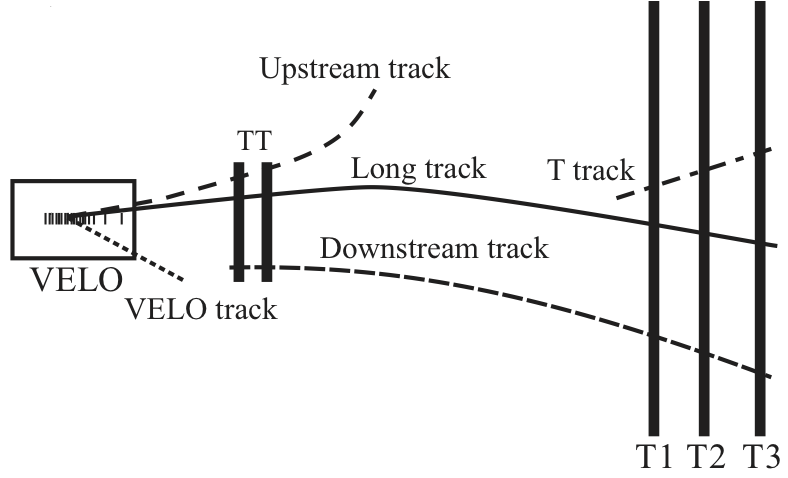
\includegraphics[width=0.48\textwidth]{track}
    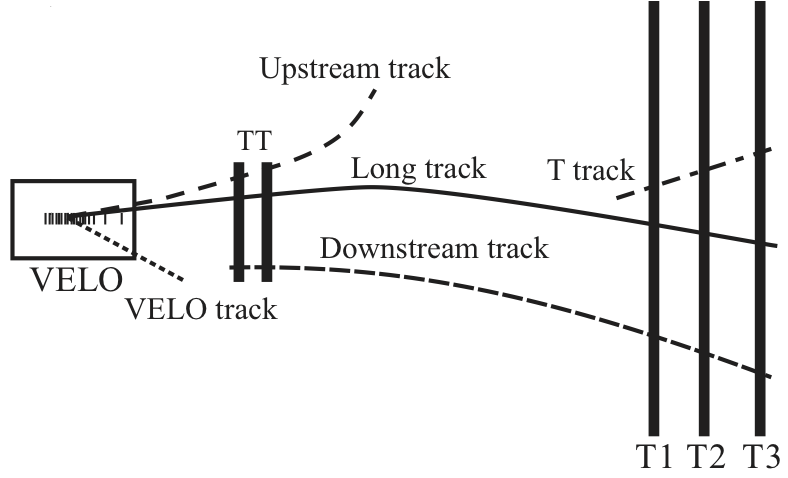
\includegraphics[scale=0.7]{track}
    \caption[Track definitions in the LHCb detector]
    {
      Schematic diagram of the \lhcb tracking system, showing the \velo, \ttracker, and tracking
      stations T1--3.
      Track types at \lhcb are defined by the regions through which they travel, as labelled in the
      diagram.
      Most tracks used in analyses are classified as long tracks, but for long-lived particles
      (such as the \KS) downstream tracks are often also used to increase statistics.
      This analysis focused on long tracks.
      %and tracking stations one, two, and three.
      %This analysis focuses on particles decaying into a pair of long tracks.
    }
    \label{fig:db:lldd}
  \end{center}
\end{figure}

%The selection
%Simulated samples are extremely important for this analysis,
%It is important to remove sources of background while leaving the invariant mass of the dimuon
%distribution smoothly varying, so that the assumption of local-linearity remains.
%In \Sec{sec:strategy} resonances are discussed, and those where $\Gamma<5\sigmam$ must be vetoed.
%For this analysis,


The offline selection criteria applied in the stripping are outlined in \Tab{tab:stripping}.
%The variable {\tt DOCA} is defined as the distance of closest approach between any two pairs of
%tracks in the candidate.
This table lists the variables \ProbNN{\pi} and \ProbNN{K} which are \MVA algorithms
giving a response $\in[0,1]$ quantifying how pion or kaon like a particle is, respectively.
The full decay chain \btokstrdb and \dbtomumu is reconstructed using a fit in which the \Bd mass is
constrained to its known value~\cite{PDG2014}.
All references to $m(\db)$, $m(\Kstar)$ or $\tau(\db)$ are to the values after this vertex fit
has been performed.

\begin{table}[ht!]
  \caption[Stripping selection]
  {
    While the \Bd mass is constrained in the fit, the selection makes a cut on the unconstrained
    mass.
    %The variable {\tt DOCA} is defined as the distance of closest approach between any two pairs of
    %tracks in the candidate.
  }
  \label{tab:stripping}
  \begin{center}
    \begin{tabularcuts}
      \Bp
      & $\chisqvtx/\ndf$          & $<$ & 25   \\
      & \chisqip                  & $<$ & 50   \\ % BPVIPCHI2
      & $\tau$                    & $>$ & 0.2 & ps  \\
      & $m$                       & $\in$ & $[4800, 5800]$  & MeV \\
      & \pt                       & $>$ & 1000    & MeV   \\
      & $\cos\theta_\mathrm{dir}$     & $>$ & 0 \\
      \littlerule
      \db
      & $\chisqvtx/\ndf$          & $<$ & 10   \\ % VCHI2DOF
      & $\chisqfd$                & $<$ & 25   \\
      & \pt                       & $>$ & 250  & MeV \\
      & DOCA                & $<$ & 0.2 & mm \\
      & DOCA \chisq         & $<$ & 25  &    \\
      \littlerule
      Tracks
      & $\chisqtrk/\ndf$          & $<$ & 3    \\
      & $\min(\chisqip)$                  & $>$ & 9    \\ % MIPCHI2DV
      & \ProbNN{\mathrm{gh}} & $<$ & 0.3  \\
      \littlerule
      $\Kp$, $\pip$
      & \pt                       & $>$ & 250  & MeV \\
      & $p$                       & $>$ & 2000 & MeV \\
      & \chisqip                  & $>$ & 9 \\
      \Kp
      & \ProbNN{K}             & $>$ & 0.1  \\
      \pip
      & \ProbNN{\pi}           & $>$ & 0.2  \\
      \mup
      & \pt                       & $>$ & 100  & MeV \\
      & {\tt PIDmu}               & $>$ & -5   \\
      & \ismuon                   & & True \\
      \bottomrule
    \end{tabularcuts}
  \end{center}
\end{table}


\subsection{Preselection}
After the stripping and triggering stages, a loose preselection is applied, cutting on both
topological and \pid quantities; all these cuts are summarized in \Tab{tab:presel}.
The topological cuts are very approximately $90\pc$ signal efficient on all simulated samples.

Cuts are applied to the \Kstar and its daughters to remove candidates that are clearly
inconsistent with the decay  \decay{\Kstarz}{\kpi}.
Firstly, It is required that the invariant mass of the \decay{\Kstarz}{\kpi} candidate has a mass
within $100\mev$ of the known mass of the $K^*(892)^0$ meson, which has been measured to be
$(895.81\pm0.19)\mev$~\cite{PDG2014}.
\pid constraints are also applied to each \Kstar daughter: $\dllkpi(\Kp)>-5$, $\dllkpi(\pip)<25$;
and to ensure that the kaon candidate looks more like a kaon than the pion candidate a cut on the
difference in \glspl{DLL} is also applied: $\dllkpi(\Kp)-\dllkpi(\pip)>10$.

The decay \decay{\KS}{\pipi} has a branching fraction of
$(69.20\pm0.05)\e{-2}$~\cite{PDG2014}, and is removed in the preselection by requiring that
$|m_{\pi_\mu^+\pi_\mu^-}-m_{\KS}^\mathrm{PDG}|<25$.
This roughly translates to a cut in the dimuon invariant mass spectrum of
$436<m_{\mumu}<490\mev$.

Since the \db can be displaced from the \Bd decay vertex, a potential background for the decay
\dbtomumu is from a \mumu pair directly from a \pv.
This is suppressed by requiring that the transverse flight distance (\FDT) of the \db vertex, with
respect to the \pv is greater than $0.1\mm$.

The high branching fraction of \decay{\Bd}{\jpsi(\to\mumu)\Kstarz} means that there is also
contamination from decays where a hadron is misidentified as a muon, and vice versa.
This background can be suppressed by requiring that neither of the \Kstarz daughters satisfy the
\ismuon criteria, the effect of this cut is shown in \Fig{fig:db:doublemisid}.
A summary of all preselection cuts is shown in \Tab{tab:db:presel}.

\begin{figure}
  \begin{center}
    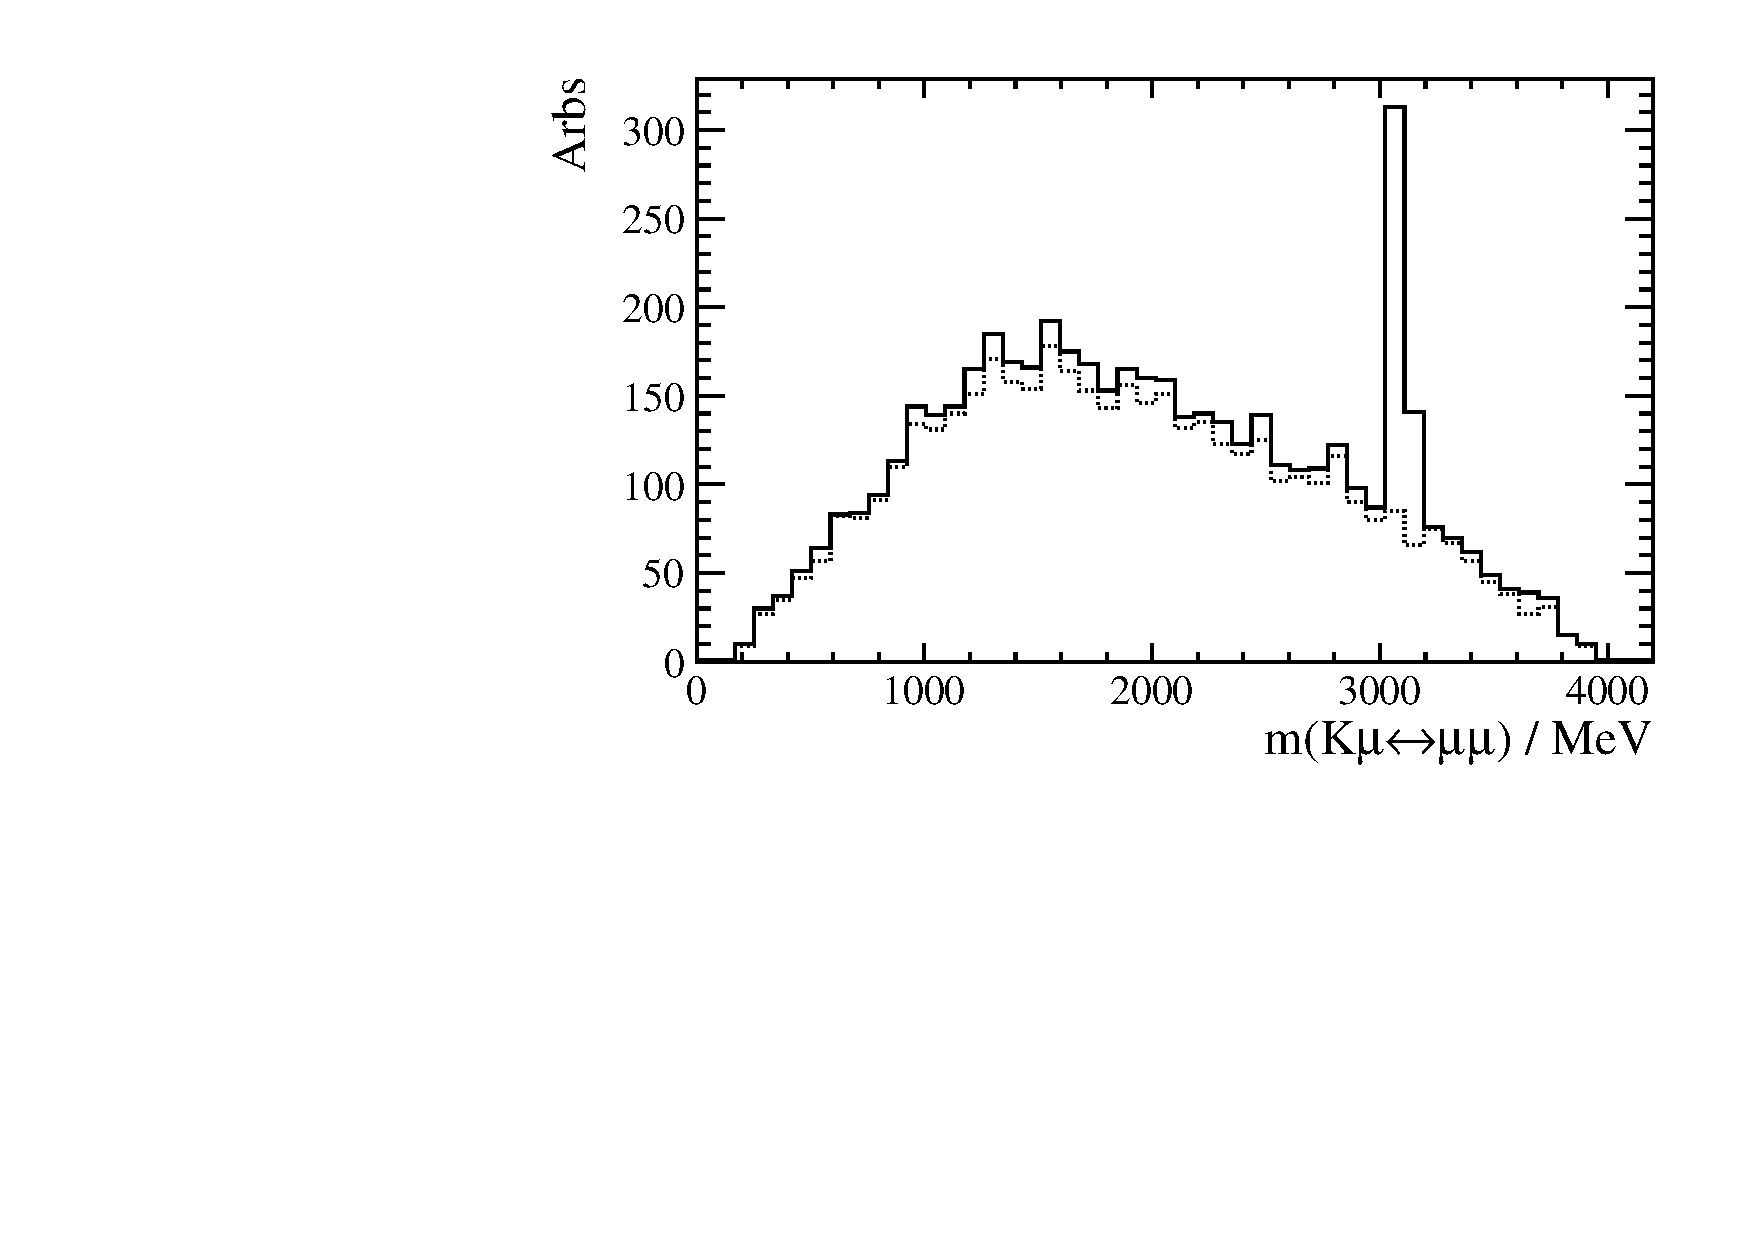
\includegraphics[width=0.48\textwidth]{double_misid_pi}
    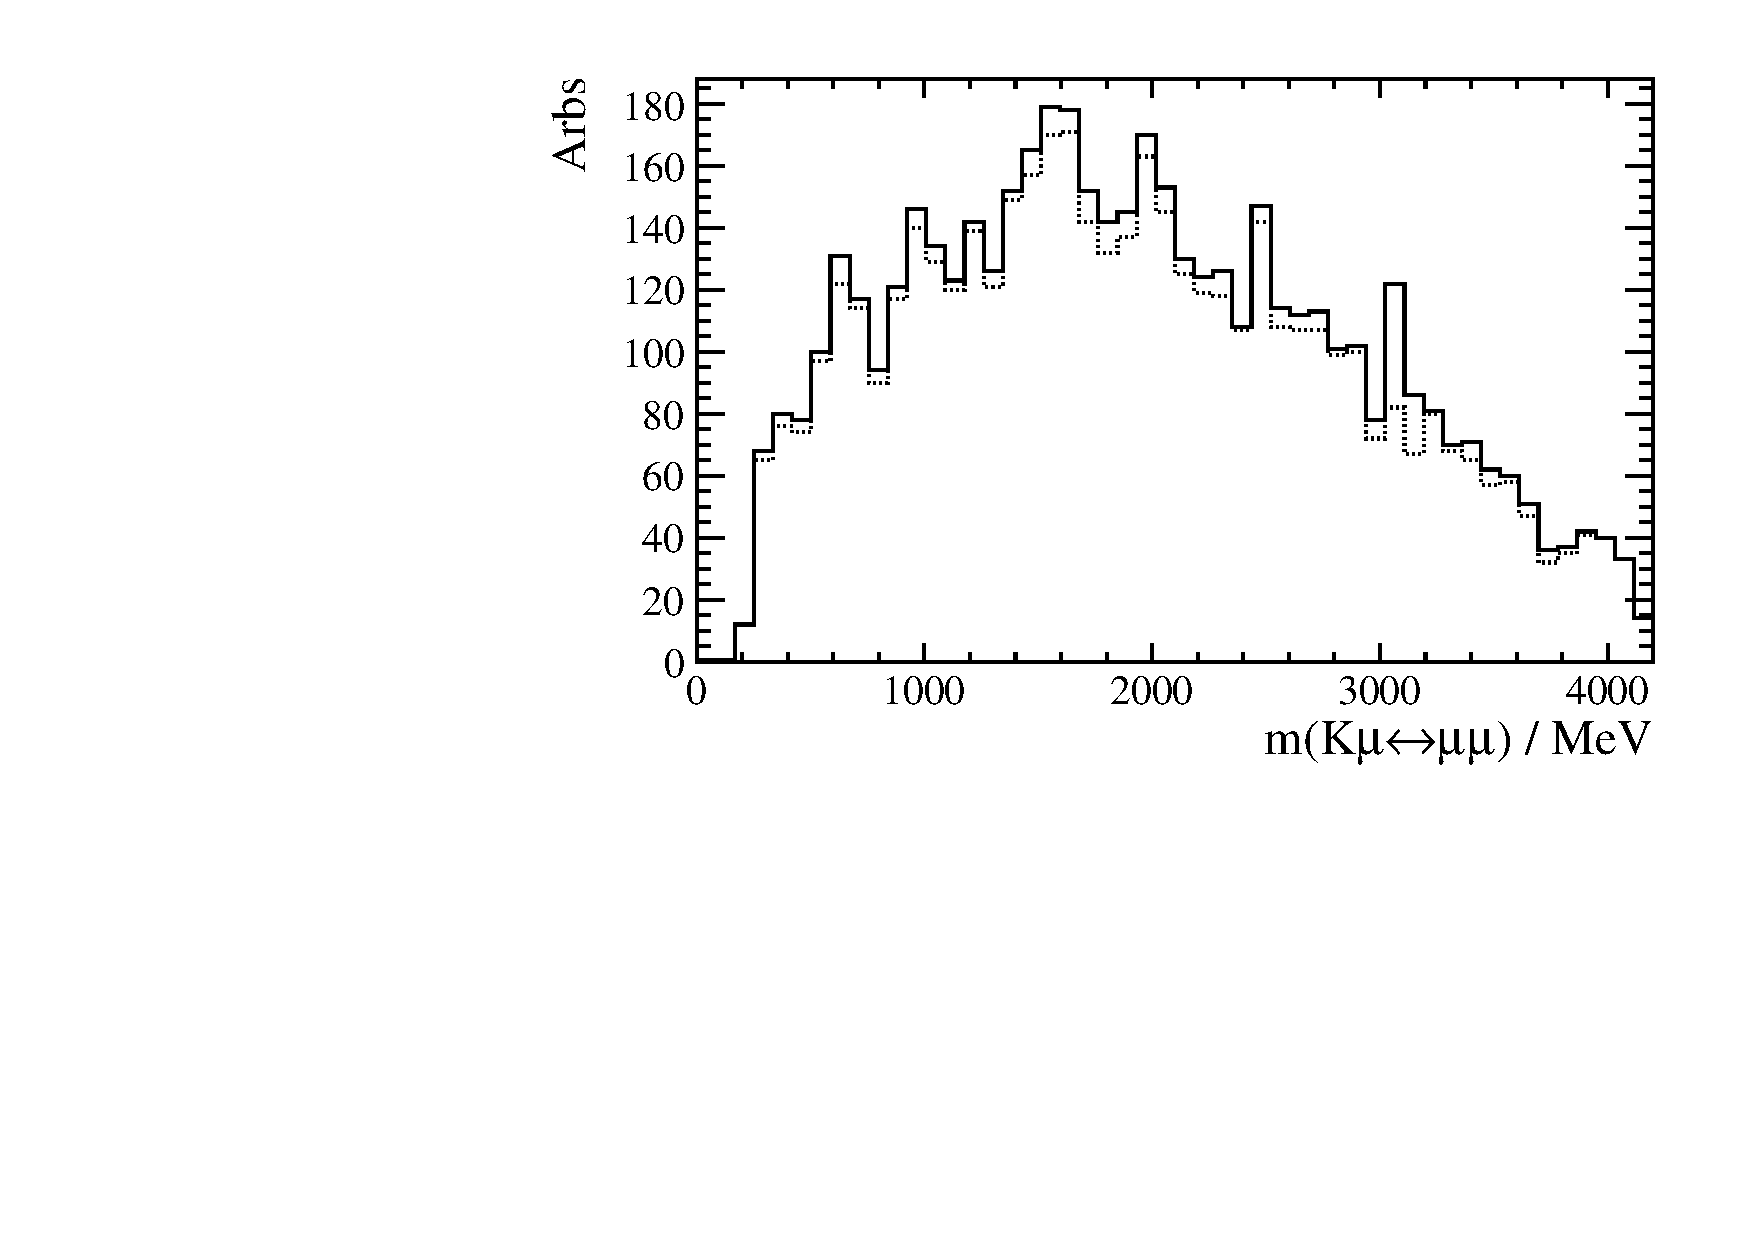
\includegraphics[width=0.48\textwidth]{double_misid_k}
    \caption[Effect of the double misidentification veto]
    {
      Double misid
    }
    \label{fig:db:doublemisid}
  \end{center}
\end{figure}

\begin{table}
  \caption[Preselection cuts]
  {
    Summary of preselection cuts applied to the \btokstrdb candidates.
  }
  \label{tab:db:presel}
  \begin{center}
    \begin{tabularcuts}
      \Bd
      & $\theta_\mathrm{dir}$ &$<$& 0.03 & rad \\
      & $\chisqvtx$ &$<$& 15 \\
      & $\chisqip$ &$<$& 10 \\\littlerule
      \Kstarz
      %& $|m_{\kpi}-895.8|$ & $<$ & 100 & MeV \\
      & $|m_{\kpi}-m_{\Kstarz}^{\pdg}|$ & $<$ & 100 & MeV \\
      & $\dllkpi(K)-\dllkpi(\pi)$ & $>$ & 10 \\\littlerule
      \Kp
      & $\ismuon$ && {\tt False} \\
      & $\dllkpi$&  $>$ & -5 \\\littlerule
      \pip
      & $\ismuon$ && {\tt False} \\
      & $\dllkpi$&  $<$ & 25 \\\littlerule
      \db
      & $F\!D_T$ & $>$ & 0.1 & mm \\
      & $m$  & $\notin$ & $[436,490]$ & MeV \\
      \bottomrule
    \end{tabularcuts}
  \end{center}
\end{table}


\subsection{Other backgrounds from particle misidentification}
\label{sec:db:backgrounds:misid}

Beyond backgrounds from onia states and the \KS decay there are many mesons that decay into a
two-body final state, which could mimic the signal decay given some particle misidentification.
A meson that decays via $\decay{X}{hh^\prime}$ which is then reconstructed
under the incorrect mass hypothesis could pass the selection criteria as either the \db or \Kstarz
candidate.
This type of contamination is studied by assigning different mass hypotheses to each final state
particle and calculating the invariant mass of the \mumu and \kpi candidates.
If the mass of one of these objects, after mass reassignment, is seen to peak at the mass of a
known particle, then the contamination is removed by applying \pid criteria.

Since a selection has been made on the \decay{\Kstarz}{\kpi} candidate using both \pid criteria and
constraints on the \kpi invariant mass it is expected that there will be little contamination
from background sources.
To test this, candidate \Kstarz mesons coming from a \Bd candidate with an invariant mass
within $80\mev$ of the known \Bd mass are assigned different mass hypotheses to check for peaking
components in the new $\mass{K_{h}^+\pi_{h^\prime}^-}$ mass spectrum.
%\footnote{
  %Where, as defined previously, the notation $h_i$ is a particle under the mass hypothesis of $h$
  %which was reconstructed as an $i$.
%}
The only background that must be removed from this category is from a real \decay{\phi}{\kk}
where a kaon in the final state is misidentified as being a pion.
If the mass of the $\Kp K^-_\pi$ candidate lies within $10\mev$ of the known \phii mass, the
ambiguous pion is subject to the requirements that
$\ProbNN{\pi}<0.3$ and $\ProbNN{K}>0.3$.

Resonances decaying into a pair of hadrons which are mistaken as a pair of
muons are more problematic.
%Misidentification of the decay \decay{\KS}{\pipi} is already dealt with in the preselection, but
Weak Decays of mesons can contribute to background, especially
\decay{\Dz}{\kpi} and \decay{\Lz}{p\pim}, which are dealt with in a similar way to the vetoes
described in \Chap{ch:dsphi}.
If the invariant mass of the $K^+_\mu\pi^-_\mu(p_\mu\pi^-_\mu)$ candidate falls within $25(10)\mev$
of the nominal $\Dz(\Lz)$ mass, then the muons are subject to the requirement that
$\ProbNN{\mu}(\Kp_\mu,\pip_\mu)>0.3(\ProbNN{p}(p_\mu)<0.3)$.


\begin{table}
  \begin{center}
    \begin{tabular}{lcc}\toprule
      \multicolumn{2}{c}{Mass criteria (MeV)} & PID requirement \\\midrule
      $\left|m(\Kp K^-_\pi) - m^\mathrm{PDG}_\phi\right|$ & $<10$
      & $\ProbNN{\pi}(\pi)>0.3$ and \ProbNN{K}$(\pi)<0.3$
      \\\rule{0pt}{3ex}$\left|m(K^+_\mu\pi^-_\mu) - m^\mathrm{PDG}_{\Dz}\right|$& $<25$
      & $\ProbNN{\mu}(\mu)>0.3$
      \\\rule{0pt}{3ex}$\left|m(p_\mu\pi^-_\mu) - m^\mathrm{PDG}_{\Lz}\right|$ & $<10$
      & $\ProbNN{p}(\mu)<0.3$
      \\\rule{0pt}{3ex}$\left|m(p_\pi K^-\mumu) - m^\mathrm{PDG}_{\Lb}\right|$ & $<50$
      & $\ProbNN{p}(\pi)<0.2$  \\
      \bottomrule
    \end{tabular}
  \end{center}
  \caption[Veto conditions to suppress backgrounds from misidentifications]
  {
   Veto conditions to suppress double and single misidentification of particles.
   If, under the alternate hypothesis, the \db or \Kstarz candidate mass falls within the range
   indicated, the candidates are subject to the given \pid requirements.
  }
  \label{tab:bkg:vetoes}
\end{table}

Misidentifying the proton as a pion in the decay \decay{\Lb}{p\Km\mumu} can contaminate the
selected \btokstrdb candidates.
Figure~\ref{fig:db:lb} shows the invariant mass distribution of the $p_\pi\Km\mumu$ system for
candidates where $\ProbNN{p}(p_\pi)>0.2$, a clear peak is observed at the known mass of the \Lb.
Candidates are removed by if the mass of the \Lb candidate falls within $50\mev$ of the
nominal \Lb mass and satisfies $\ProbNN{p}(p_\pi)>0.2$.


\begin{figure}
  \begin{center}
    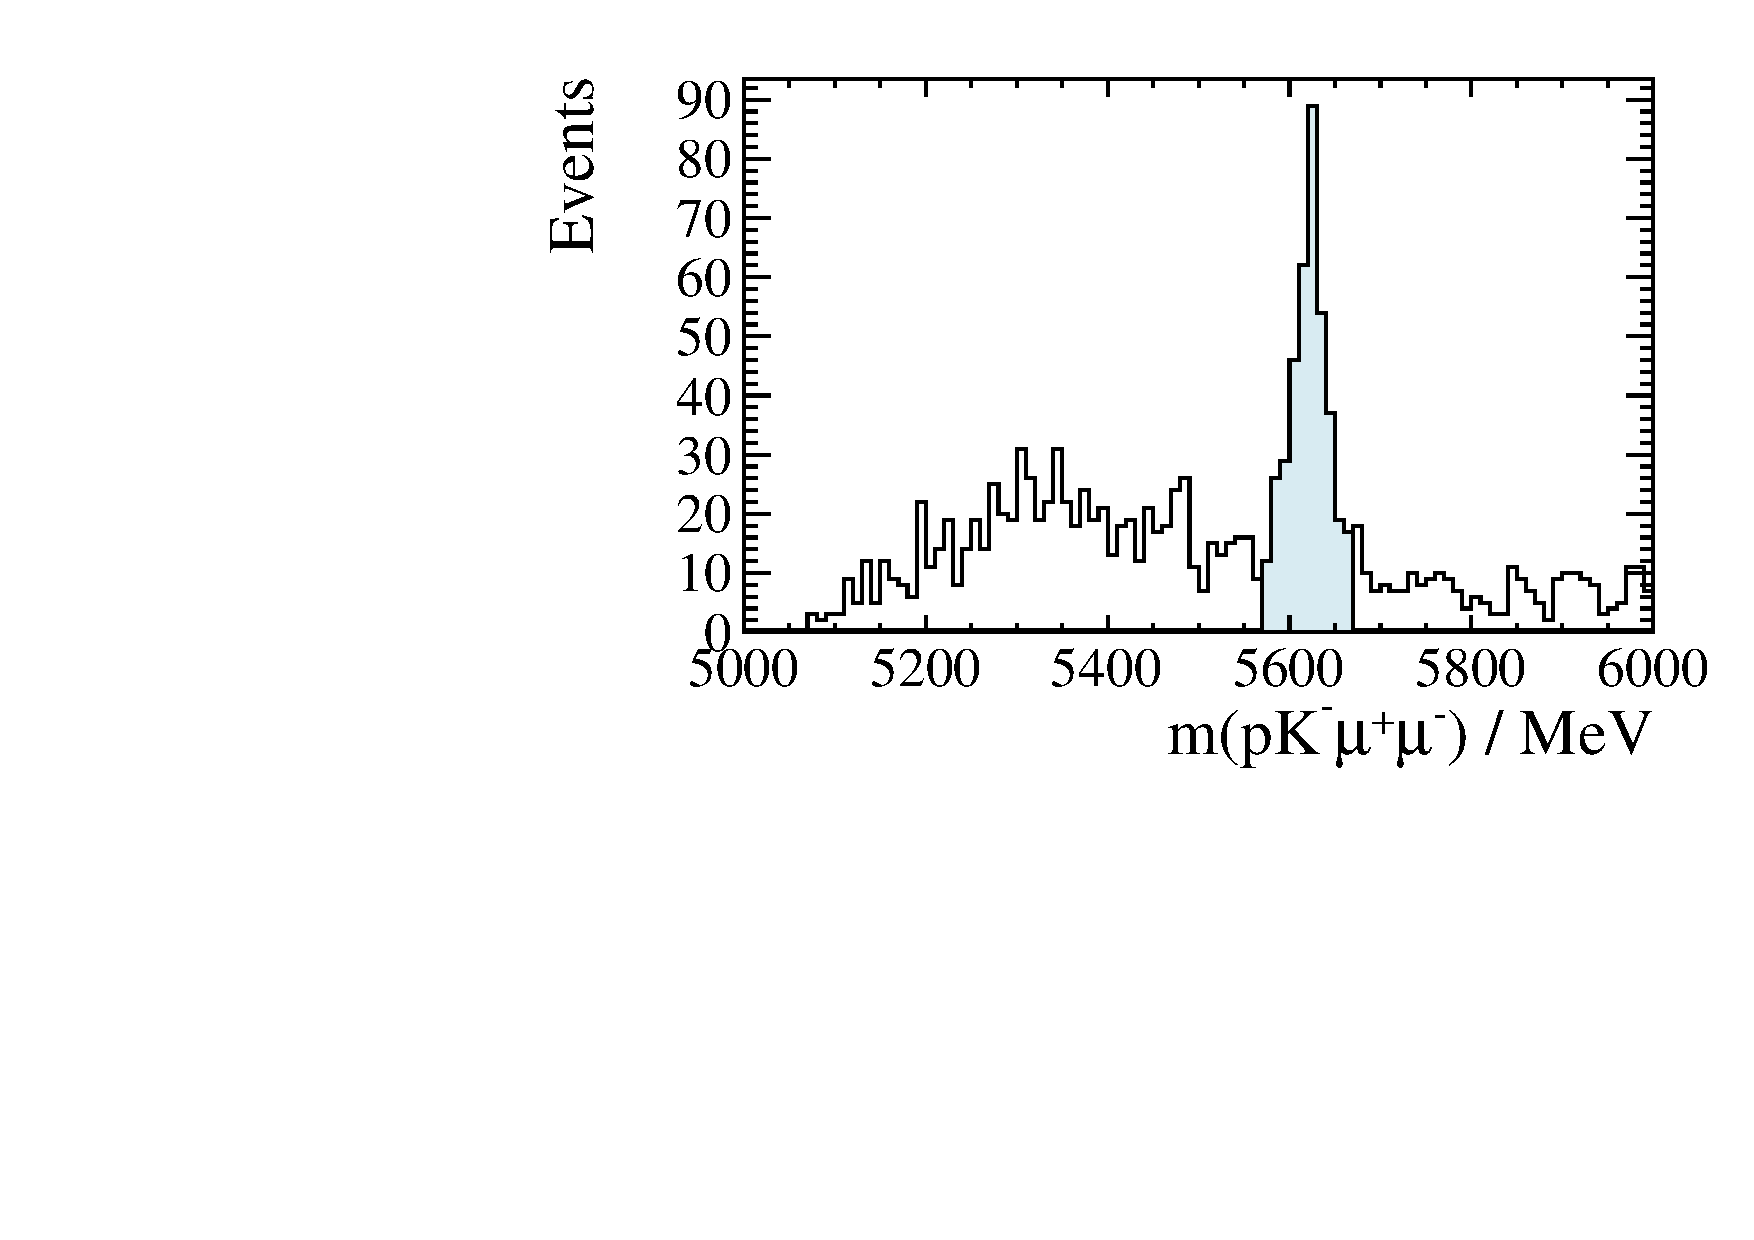
\includegraphics[width=0.48\textwidth]{lb2pkmumu}
    \caption[Contamination from the decay \decay{\Lb}{p\Km\mumu}]
    {
      Contamination from the decay \decay{\Lb}{p\Km\mumu}, where the proton is misidentified as a
      pion, here a cut of $\ProbNN{p}(p_\pi)$ has been applied and a clear peak at the known \Lb
      mass, $5219.4\mev$, is observed.
      Candidates are vetoed if they lie within $50\mev$ of the \Lb mass, which is shown as the
      shaded region.
    }
    \label{fig:db:lb}
  \end{center}
\end{figure}

%There are also contributions from the decay \decay{\Bd}{\jpsi\Kstarz} and \decay{\jpsi}{\mumu},
%where one of the hadron is misidentified as a muon, and vice versa.
%This can be trivially removed by requiring that the hadrons do not satisfy {\tt isMuon}, as shown
%in \Fig{fig:bkg:doublemisid}.

%\begin{figure}
  %\begin{center}
    %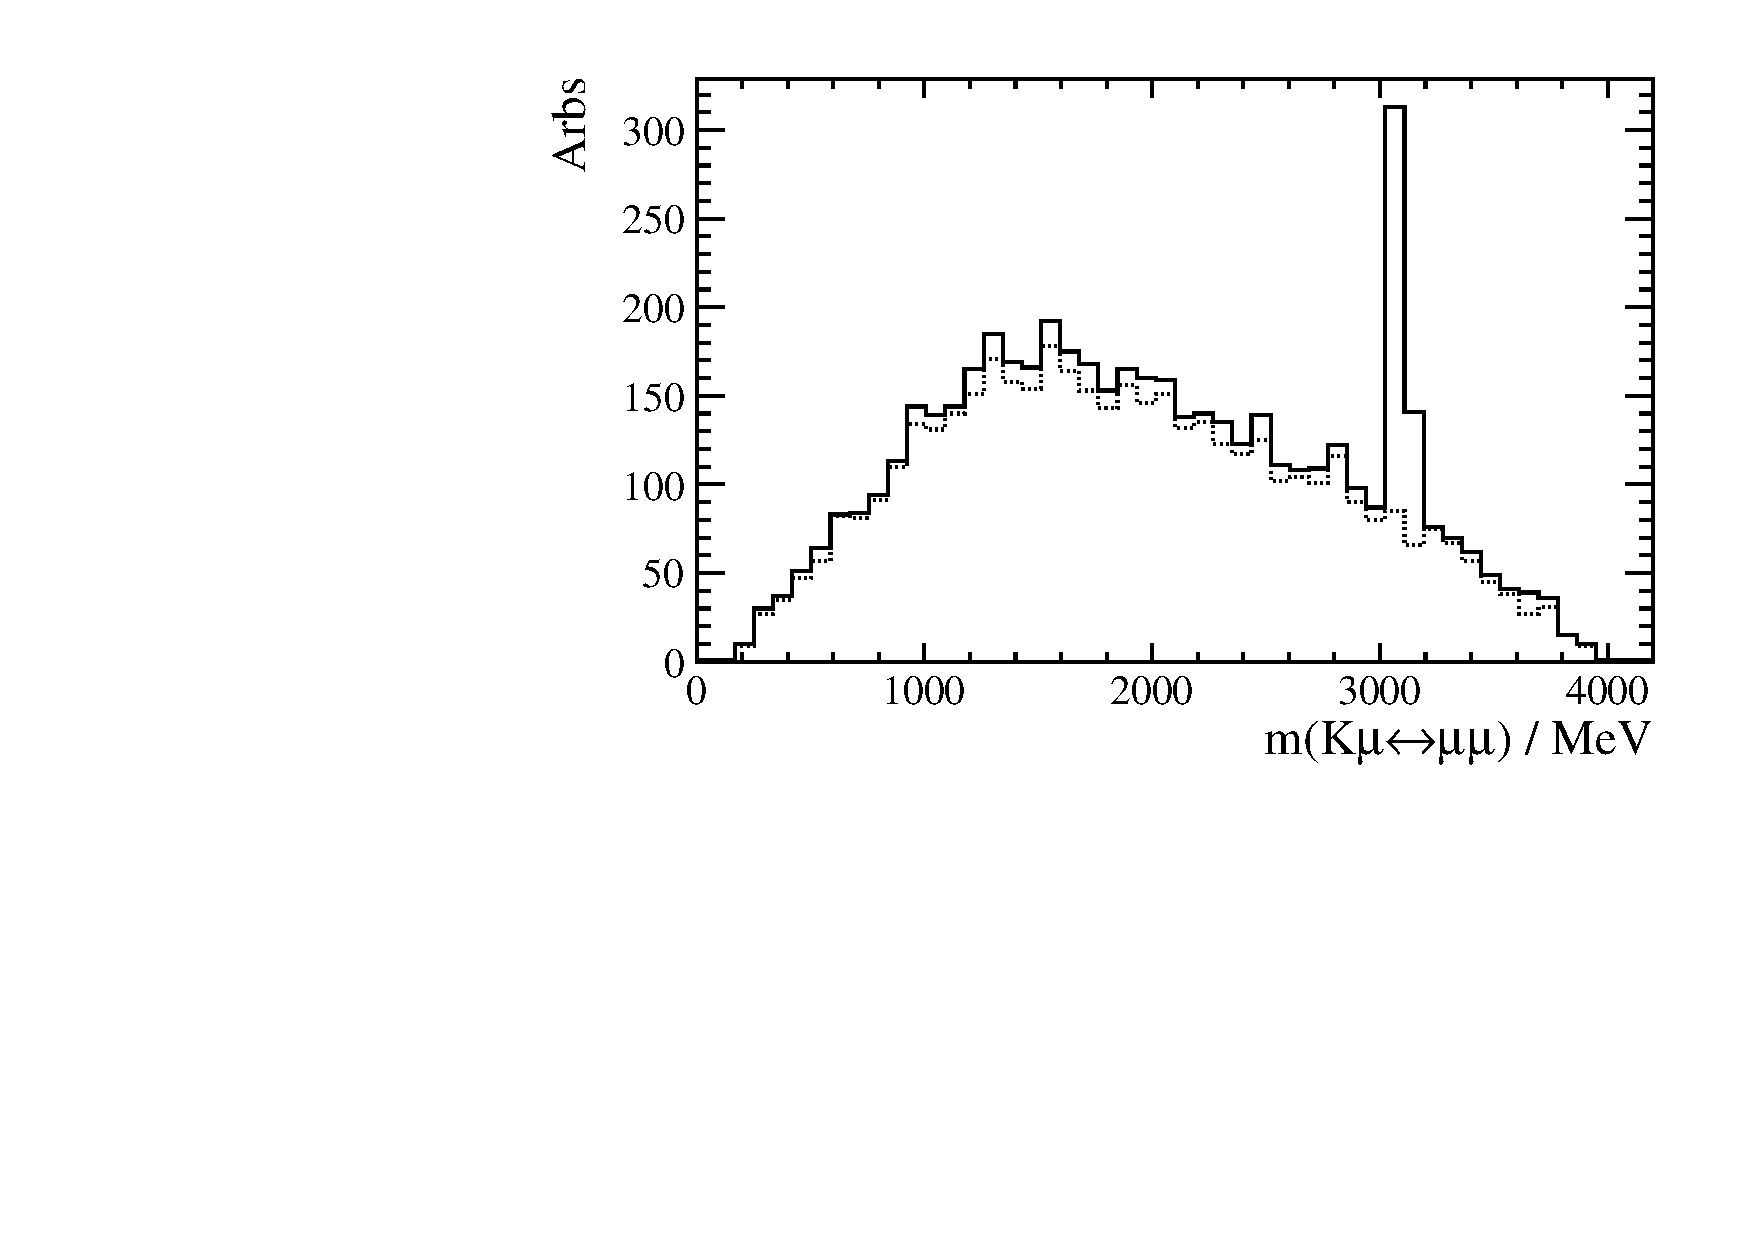
\includegraphics[width=0.48\textwidth]{double_misid_pi}
    %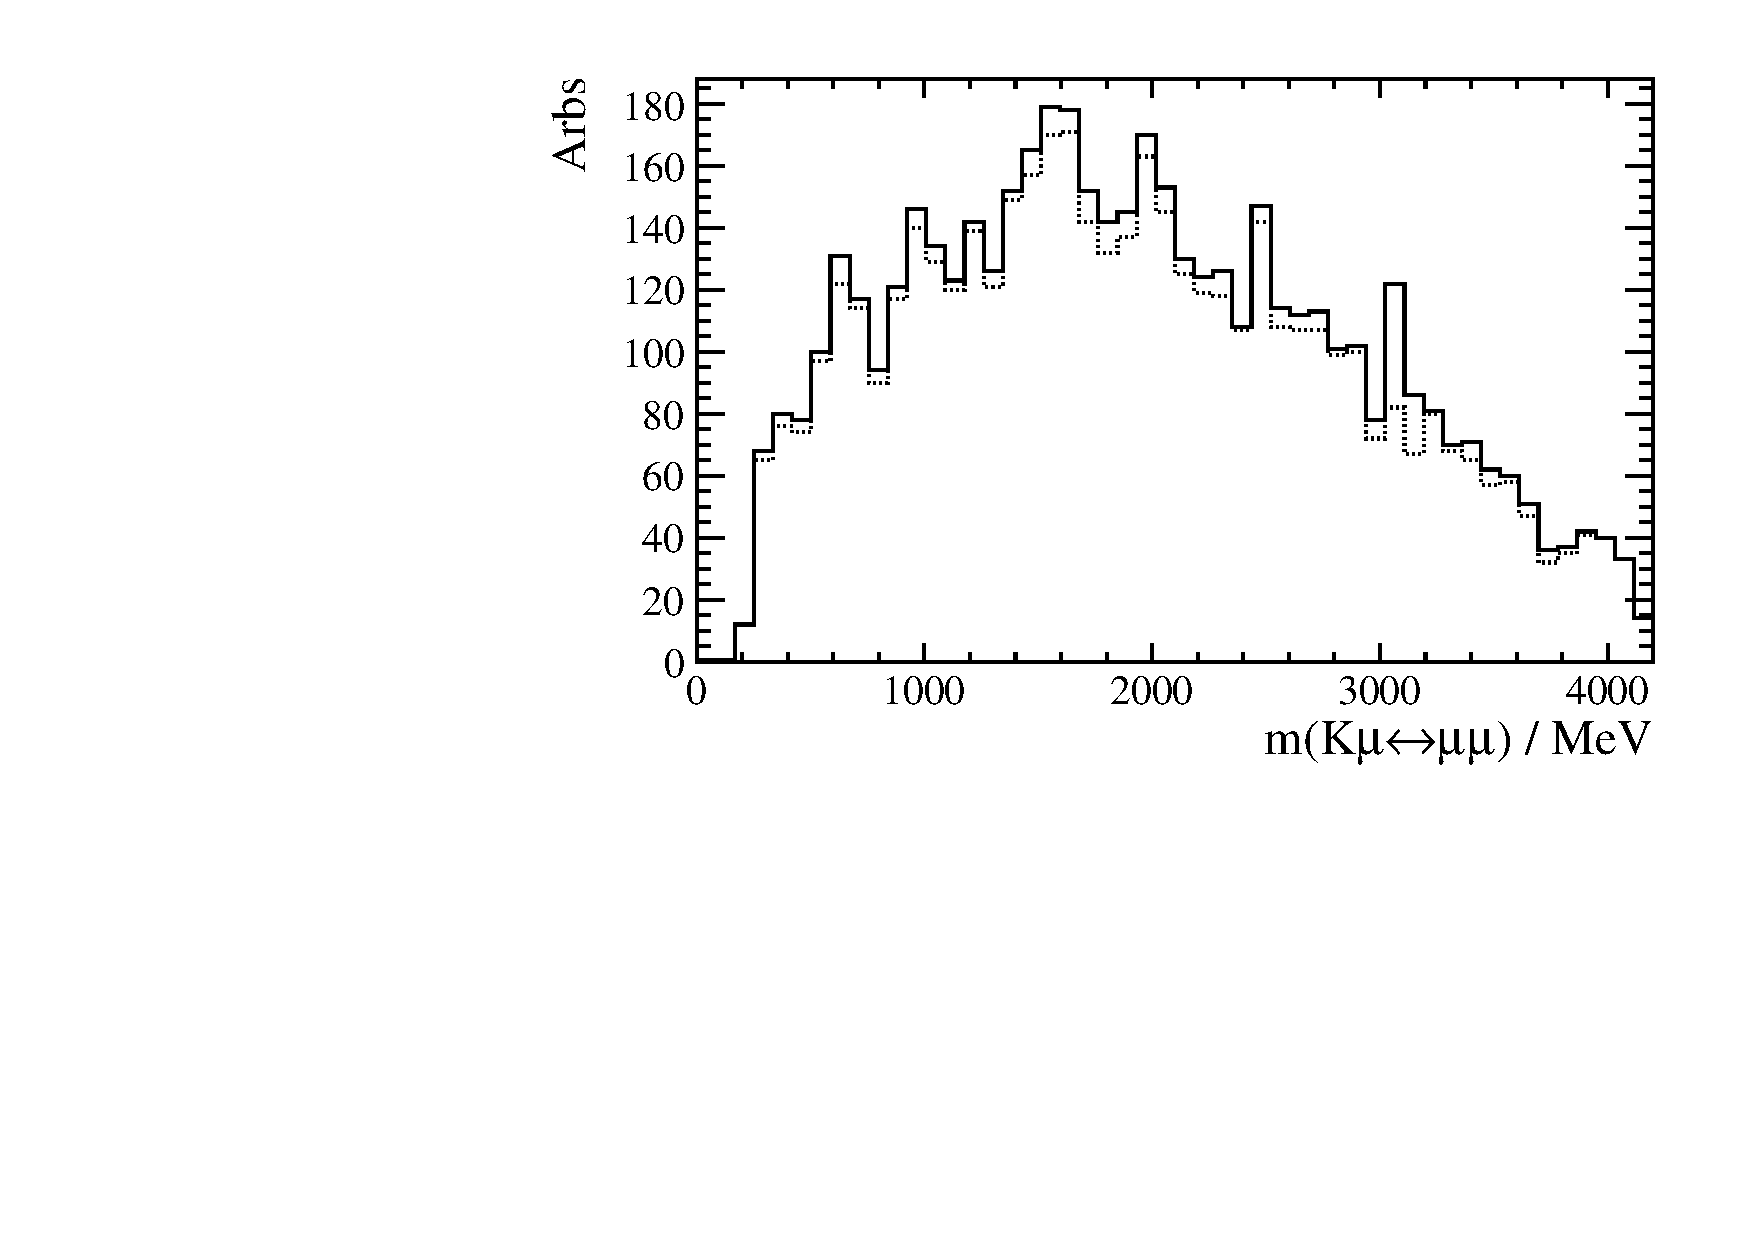
\includegraphics[width=0.48\textwidth]{double_misid_k}
    %\caption{\small
      %Background contributions from \decay{\Bd}{\jpsi\Kstarz}, where both a muon and (left) pion
      %and (right) kaon are misidentified as one another.
      %This background is very effectively removed by requiring that the hadron does not satisfy the
      %{\tt isMuon} criteria; the effect of this veto is shown with a dotted line.
    %}
    %\label{fig:bkg:doublemisid}
  %\end{center}
%\end{figure}

The sidebands are used to estimate the level of background in the signal region.
Therefore, background
contributions are only problematic if they produce a narrow peaking structure in the dimuon mass,
because misidentification causes the $m_{\mumu}$ distribution to be smeared.
In general, misidentification is only problematic if the decaying particle has a very narrow
natural width, so any remaining misidentification-type backgrounds have a negligible effect in the
analysis.


%%%%%%%%%%%%%%%%%%%%%%%%%%%%%%%%%%%%%%%%%%%%%%%%%%%%%%%%%%%%%%%%%%%%%%%%%%%%%%%%%%%%%%%%%%%%%%%%%%
\subsection[Possible contamination from the \xtsvty]
{Possible contamination from the $\boldsymbol{\xtsvty}$}
\label{sec:x1070}
%%%%%%%%%%%%%%%%%%%%%%%%%%%%%%%%%%%%%%%%%%%%%%%%%%%%%%%%%%%%%%%%%%%%%%%%%%%%%%%%%%%%%%%%%%%%%%%%%%
While searching for potential backgrounds resulting from misidentifying two hadrons as muons, a
peak is observed in the invariant mass spectrum of the $K_\mu^+K_\mu^-$ candidates.
This peak was consistent with the \xtsvty listed in \Ref{PDG2014}, which has a mass of
$(1072\pm1)\mev$ with a width of $(3.5\pm0.5)\mev$ and was observed in the $\KS\KS$ distribution
from a pion beam interacting with a liquid hydrogen target~\cite{x1070vlad}.
%from $\pim p \to \KS \KS n m\piz$ collisions~\cite{x1070vlad}, where $m\in\mathbb{Z}$.
%Figure~\ref{fig:x1070} shows the observation of this resonance from \Ref{x1070vlad} alongside
%the data from this analysis.

\begin{figure}
  \begin{center}
    %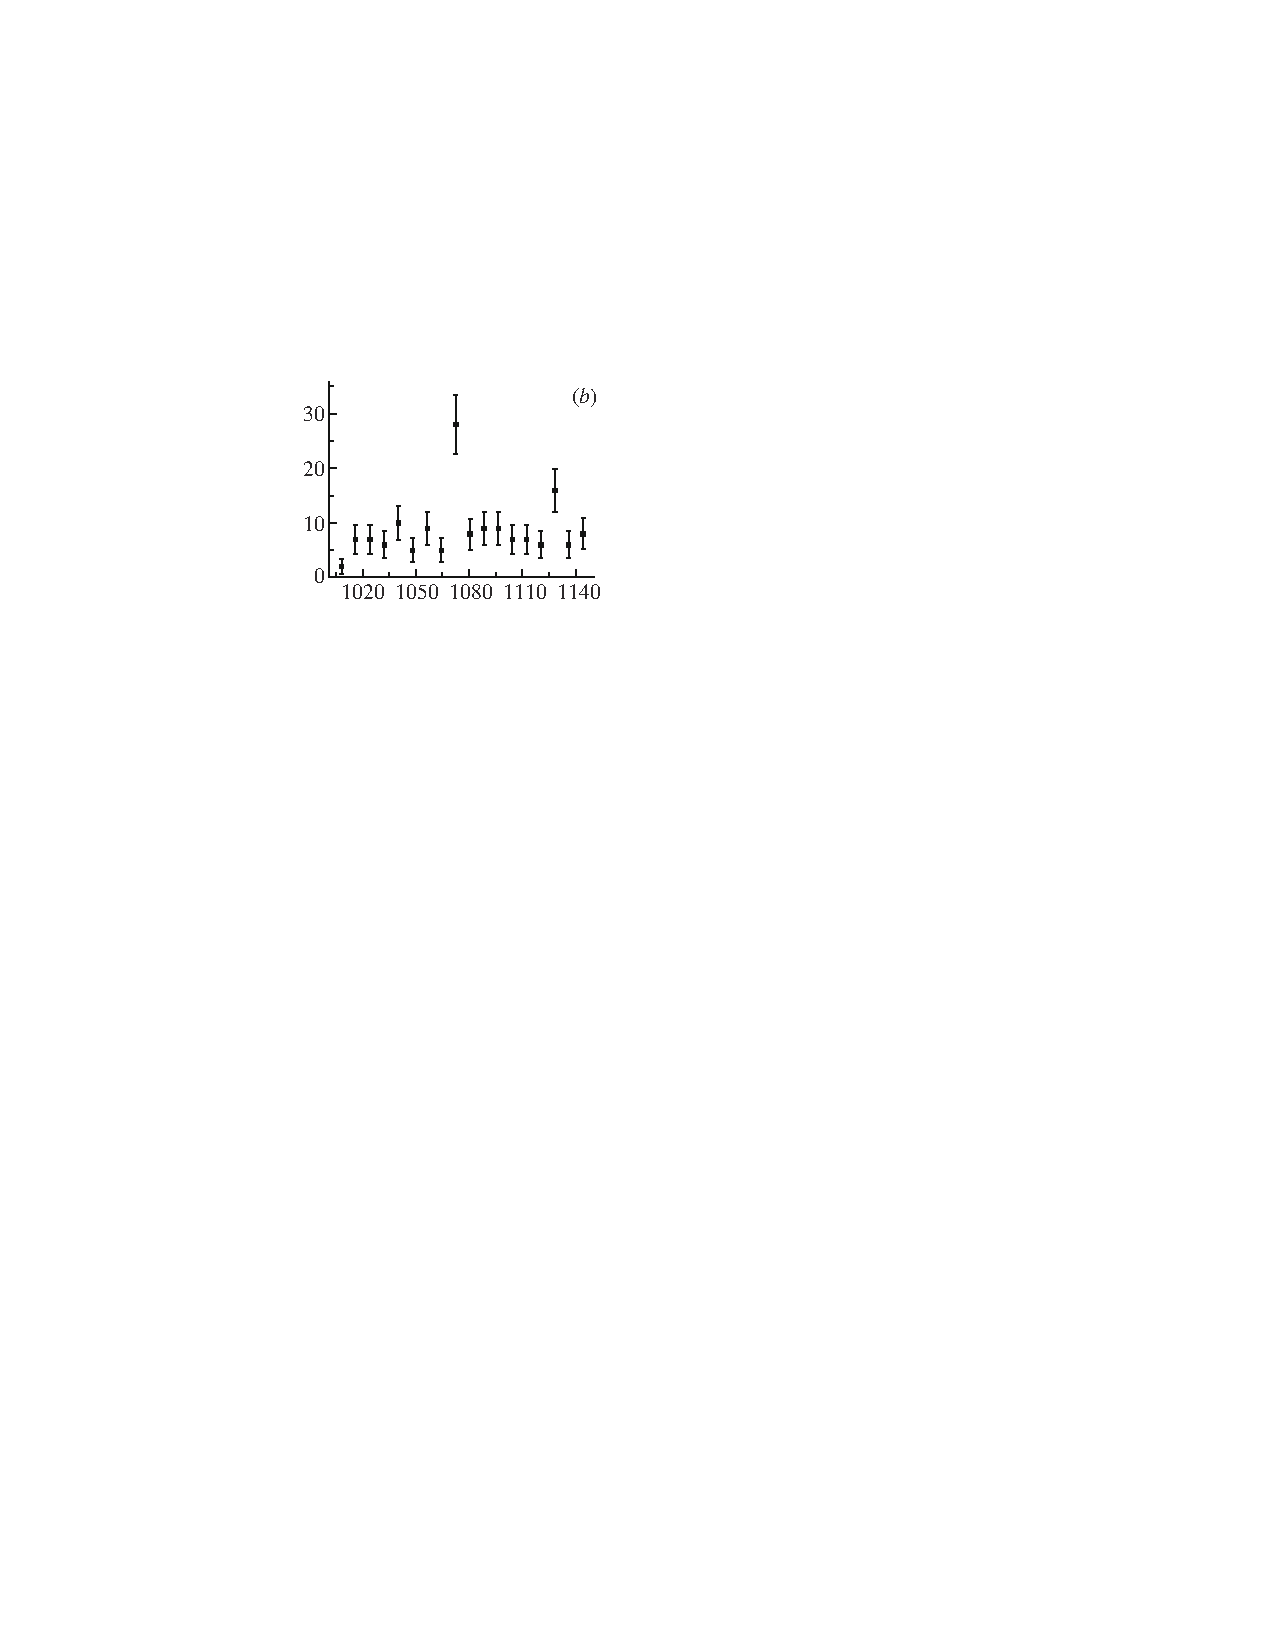
\includegraphics[height=0.2\textheight]{x1070vlad}
    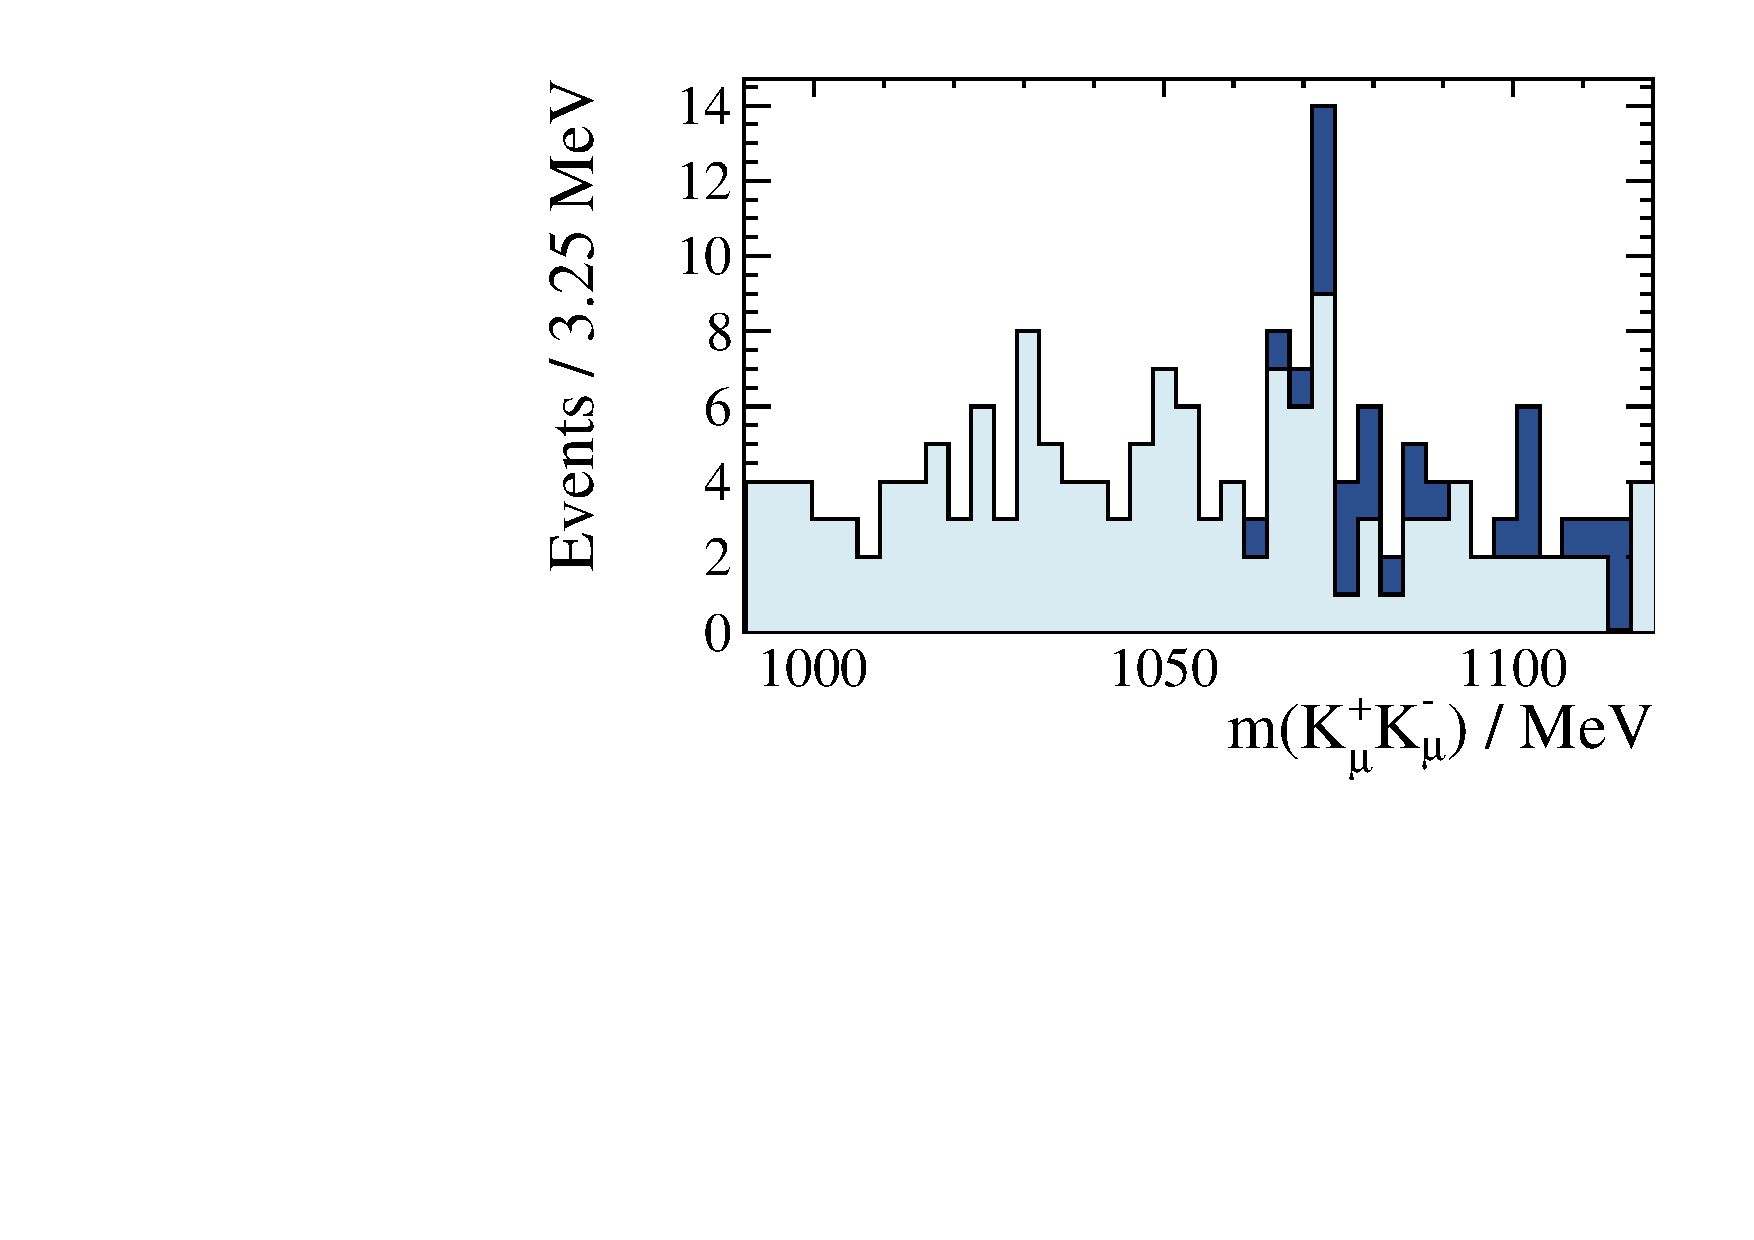
\includegraphics[height=0.2\textheight]{mumu_kk}
    \caption[Invariant mass of the \mumu distribution under the \kk mass hypotheses]
    {
      %A comparison of
      %(left) the data which observes the \xtsvty~\protect\cite{x1070vlad}, and
      Invariant mass distribution of the $K_\mu^+K_\mu^-$ candidates in data, showing a peak at
      \approx$1072\mev$ in data.
      The dark and light blue regions show the distribution before and after vetoing the decay
      \decay{\KS}{\pip\pim} in the preseletcion.
    }
    \label{fig:x1070}
  \end{center}
\end{figure}


Initially the \mumu pair under the \kk mass hypothesis appears to have a contribution from a
decaying \xtsvty.
Figure~\ref{fig:db:x1070:2d} shows a comparison of simulated \decay{\KS}{\pipi} decays with the
observed data near this excess.
It is clear that \decay{\KS}{\pipi} decays produce a peak around $1072\mev$ under the \kk
hypothesis.
There is also a long tail but with low statistics and with a roughly uniform
background this tail would not be expected to be visible in the data after the \KS veto in the
preselection.

It is clearly not the case that the $X(1070)$ is causing the peak at $m_{K^+_\mu
K^-_\mu}=1072\mev$, which is actually due to the decay \decay{\KS}{\pipi}.
Removing events satisfying $|\mass{\pi_\mu^+\pi_\mu^-}-m_{\KS}^\mathrm{PDG}|<25\mev$ removes much
of the peak at $1072\mev$, bringing it in line with the background.
Also, the fact that no \decay{\phi}{\kk} is observed in the $m_{K^+_\mu K^-_\mu}$ spectrum, and
that the peak is narrower than the resolution of the \lhcb detector,
indicate that there this is a false peak and need not be accounted for further.

\begin{figure}
  \begin{center}
    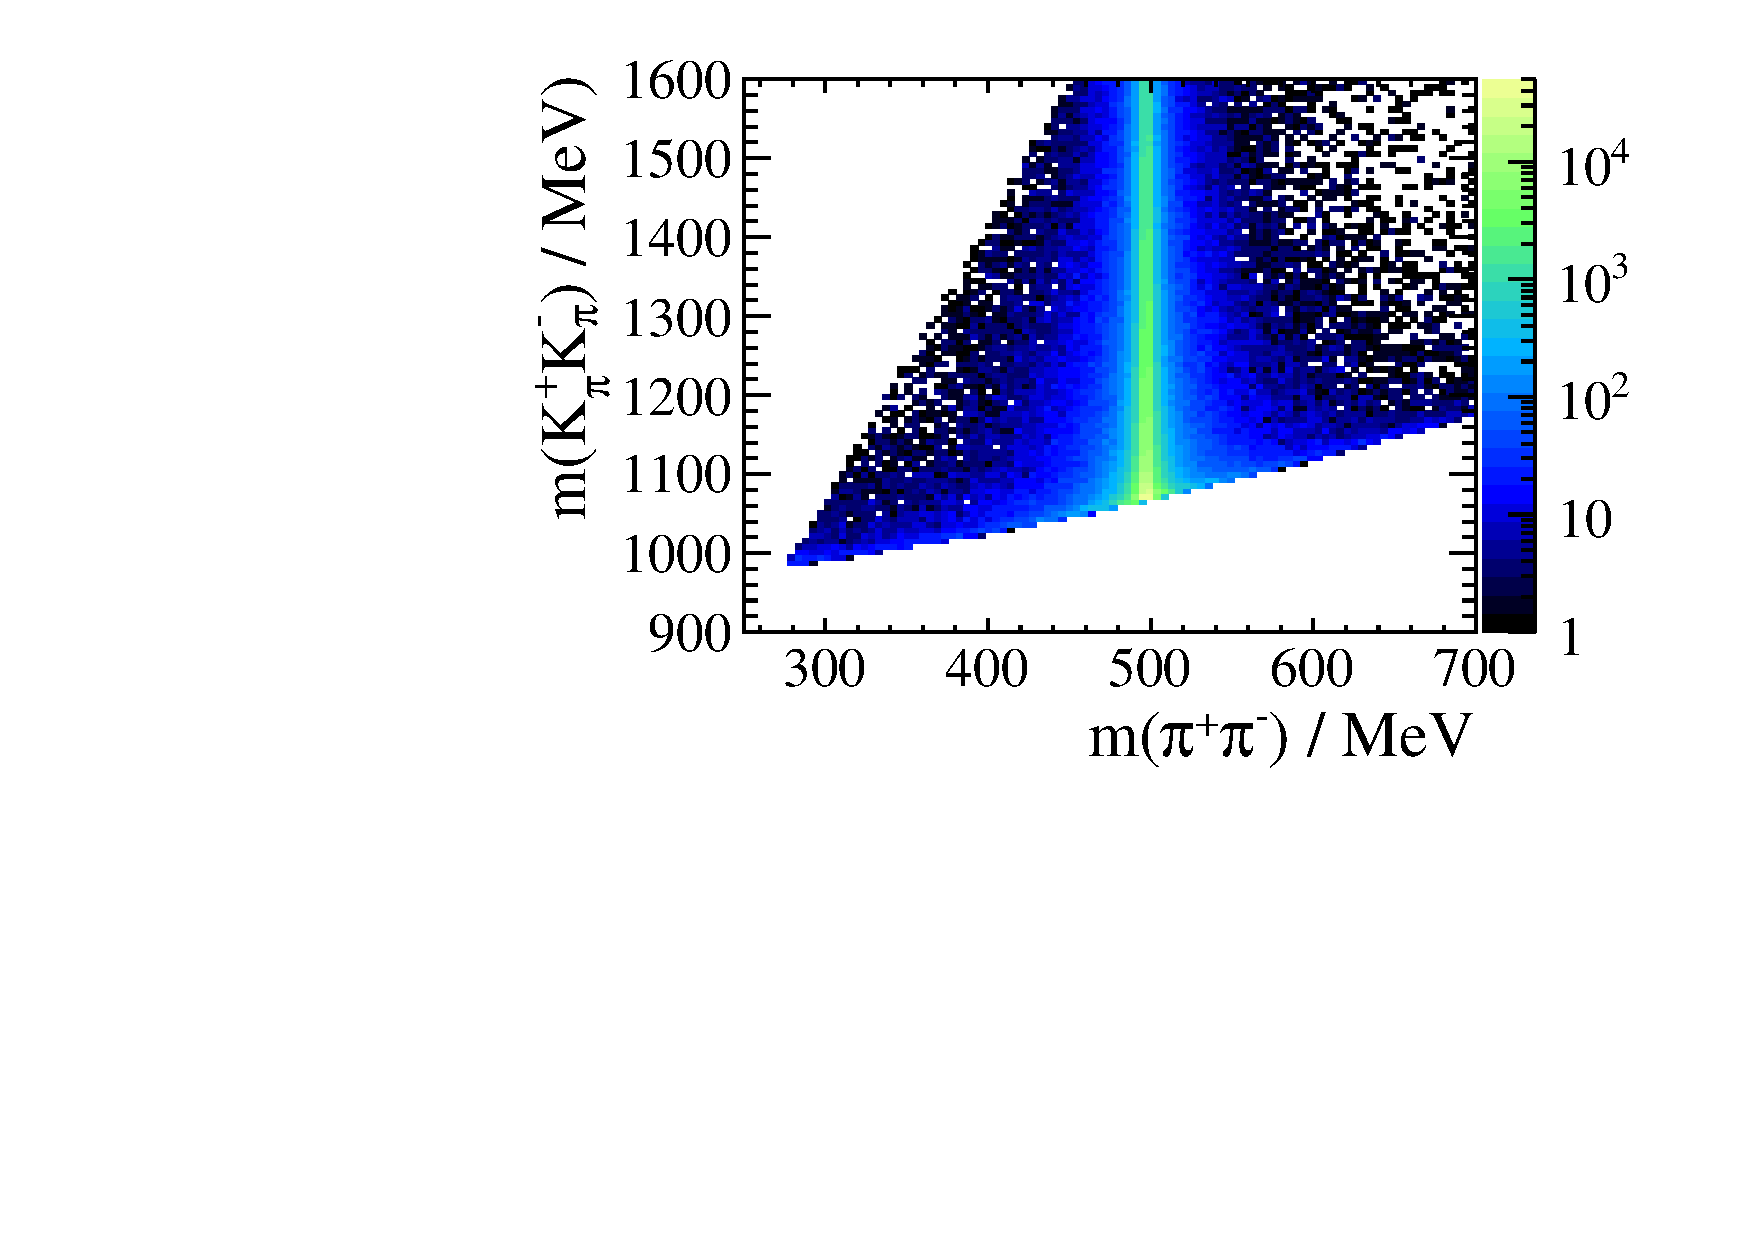
\includegraphics[width=0.48\textwidth]{gen_kk_pipi}
    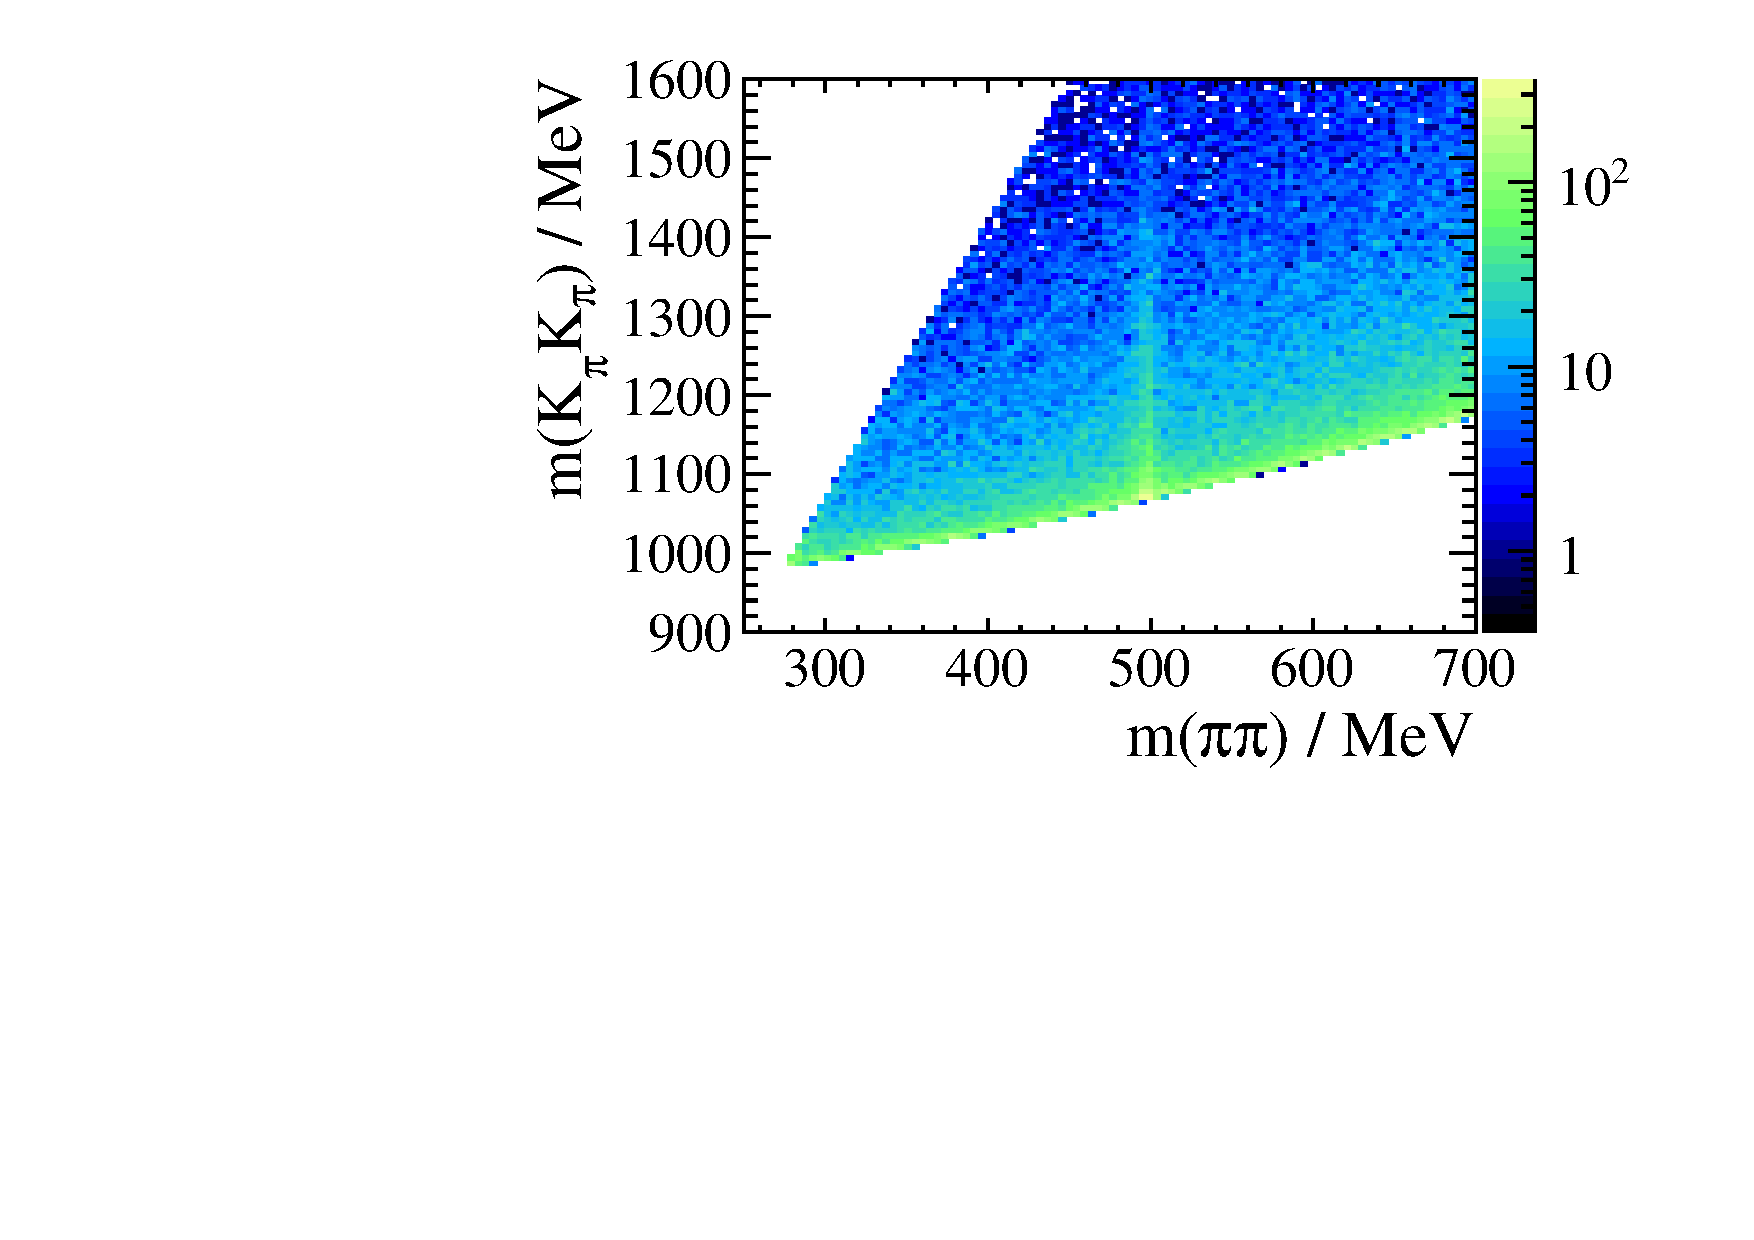
\includegraphics[width=0.48\textwidth]{data_kk_pipi}\\
    %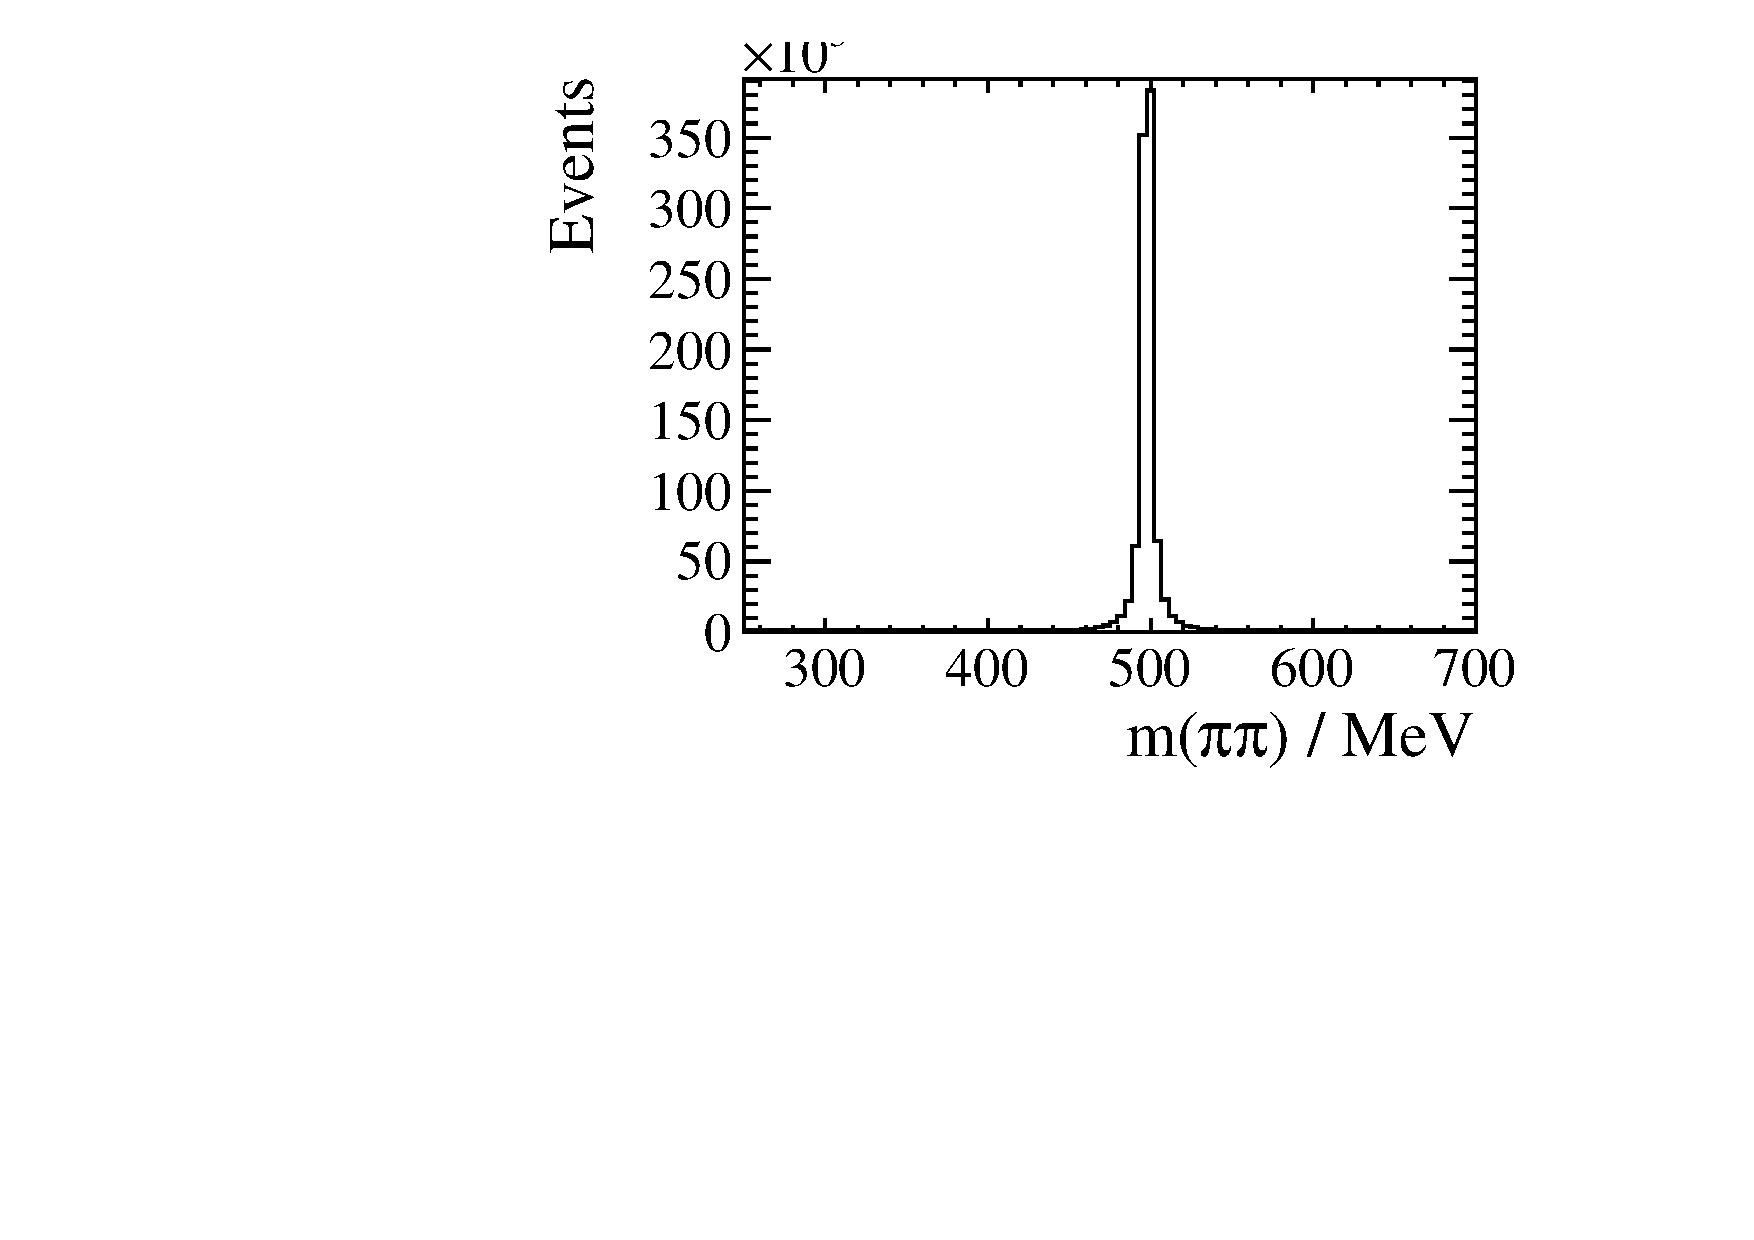
\includegraphics[width=0.48\textwidth]{gen_pipi}
    %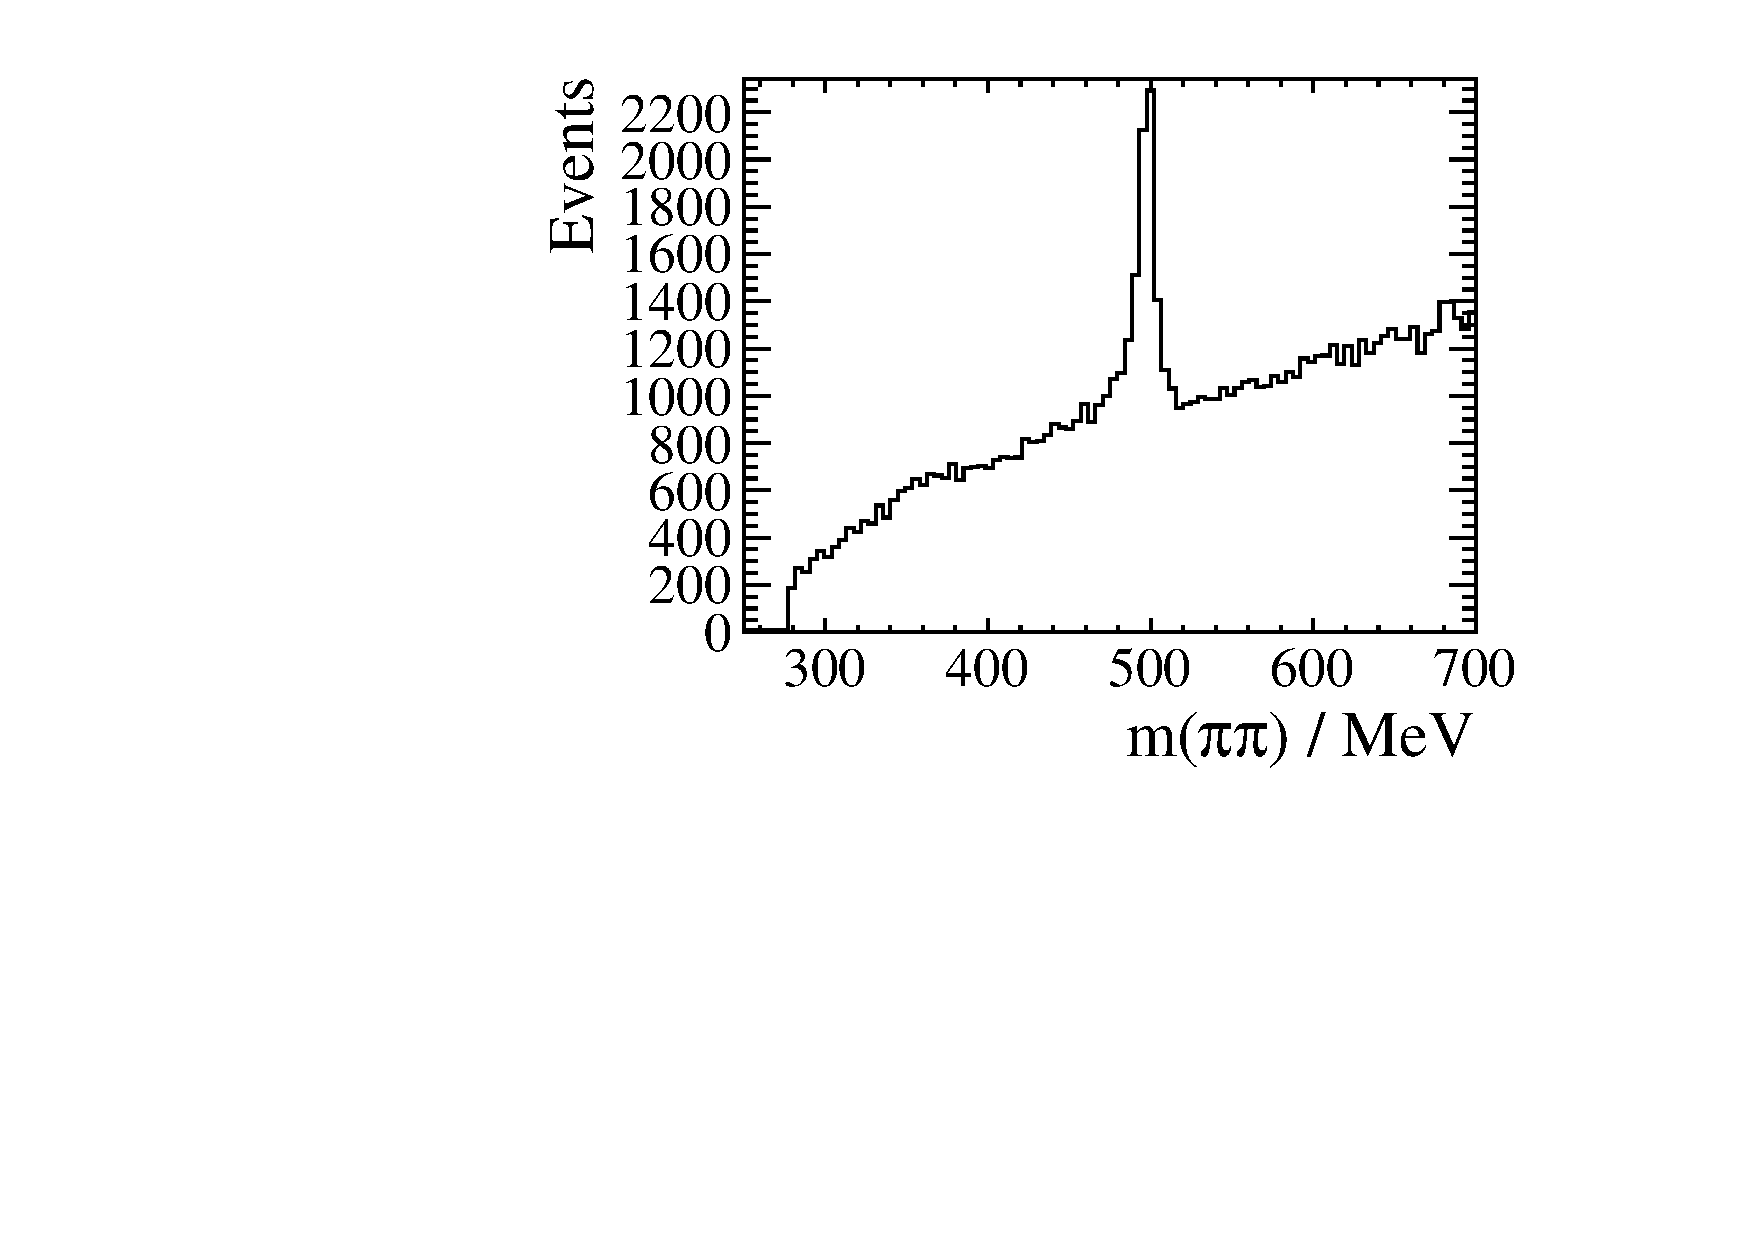
\includegraphics[width=0.48\textwidth]{data_pipi}\\
    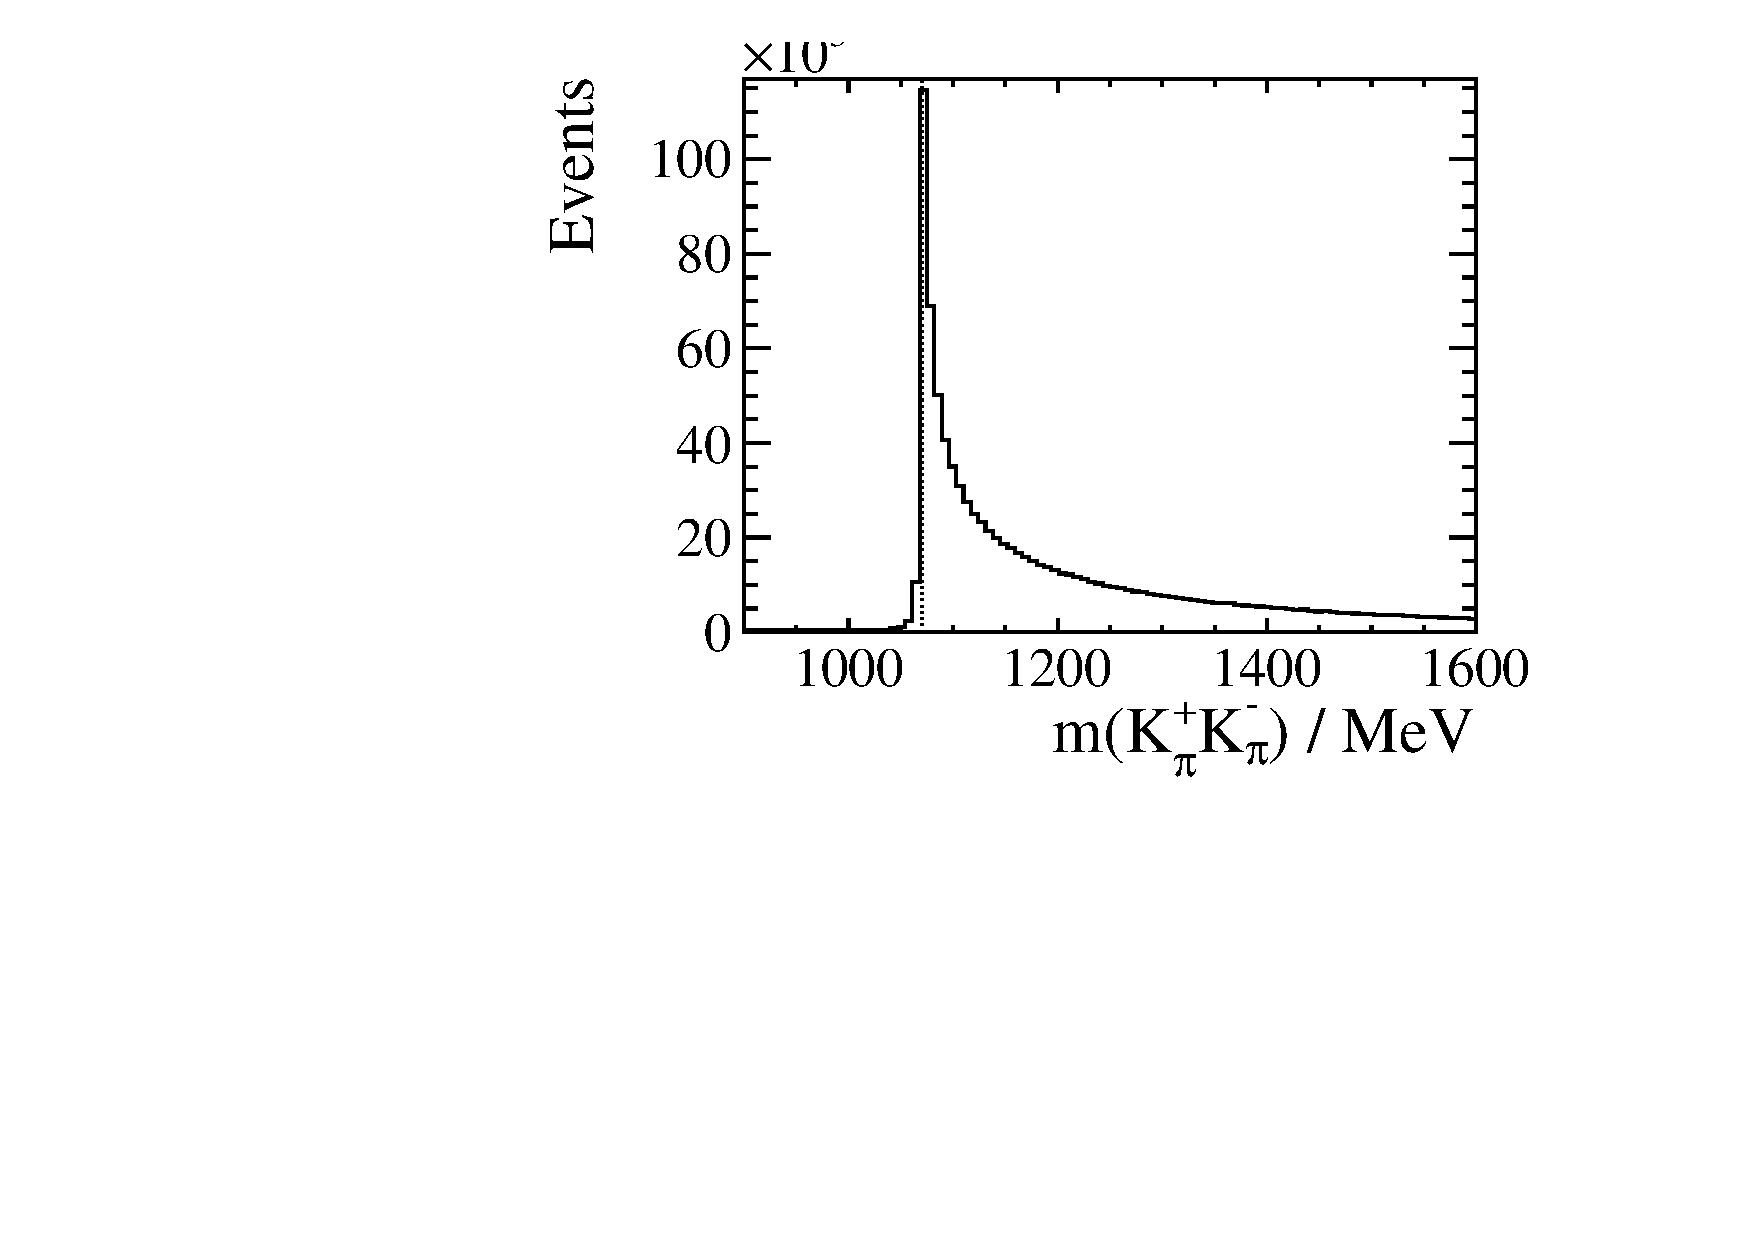
\includegraphics[width=0.48\textwidth]{gen_kk}
    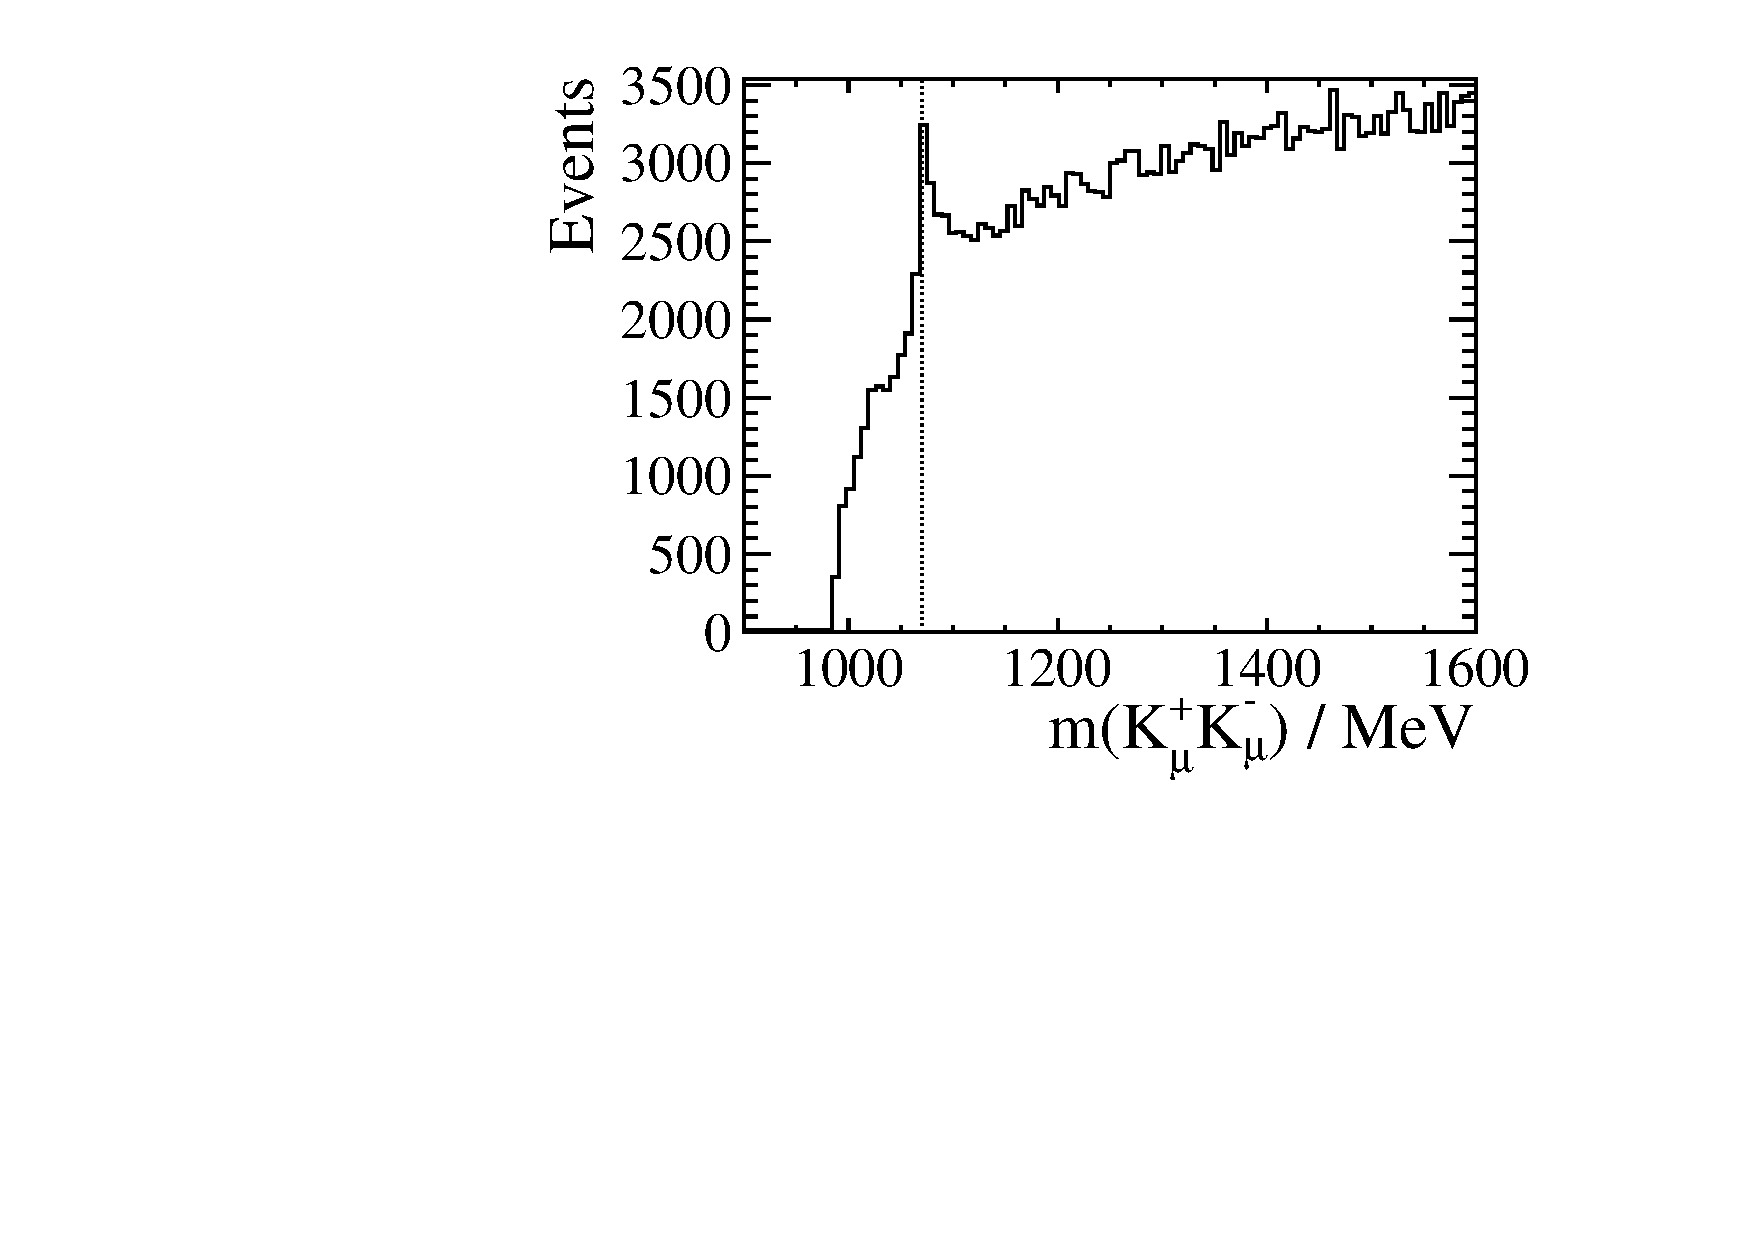
\includegraphics[width=0.48\textwidth]{data_kk}
    \caption[Analysis of the \decay{\KS}{\pipi} background under the \kk mass hypothesis]
    {
      A comparison of \decay{\KS}{\pi\pi} under different mass hypotheses, for
      (left) simulated events, and
      (right) events from data.
      The (top) plots show the two dimensional distributions of the invariant mass distributions of
      a \pipi pair and the same candidates in the \kk mass hypothesis, the (bottom)
      plots show the projections of the \kk systems.
      Vertical lines in the lower plots indicate $1072\mev$.
    }
    \label{fig:db:x1070:2d}
  \end{center}
\end{figure}





\subsection{Multivariate selection}
The data sample is purified from combinatorial background using a multivariate selection technique.
Section \ref{sec:uboost} outlines the \uBDT algorithm, which trains a \BDT whereby events are
boosted not only based on misclassification, but also on how uniform the local response of the \BDT
is for a give set of variables.
For the case of this analysis, it is important that the \BDT does not bias the sample towards a given mass and
lifetime, which makes the \uBDT ideal for this analysis.
That being said, the uBoost algorithm should not be used at the expense of the performance of the
\BDT.
It is observed that the \uBDT algorithm in fact outperforms the AdaBoost algorithm in this case,
and therefore its use is justified.

A \uBDT is trained using a signal-proxy from simulated events and background taken from the upper
\Bd mass sideband where the \Bd candidate has a mass of over $150\mev$ above the nominal \Bd mass.
Specifically, the signal-proxy is a concoction of three different simulated samples in which the
\db has a mass of: 214, 1000, and $4000\mev$; and each has a lifetime of $100\ps$.
These samples are chosen to give the \uBDT algorithm input the largest range of masses possible.
%The fact that each sample has the same lifetime is unimportant, because $\lifetime{\db}=100\ps$ is
%sufficiently long for there to be a range of lifetimes in the signal-proxy sample.
Figure~\ref{fig:db:bdtflat} shows the effect of the uniform boosting, and that the efficiency for
all masses and lifetimes are approximately flat.

\begin{figure}
  \begin{center}
    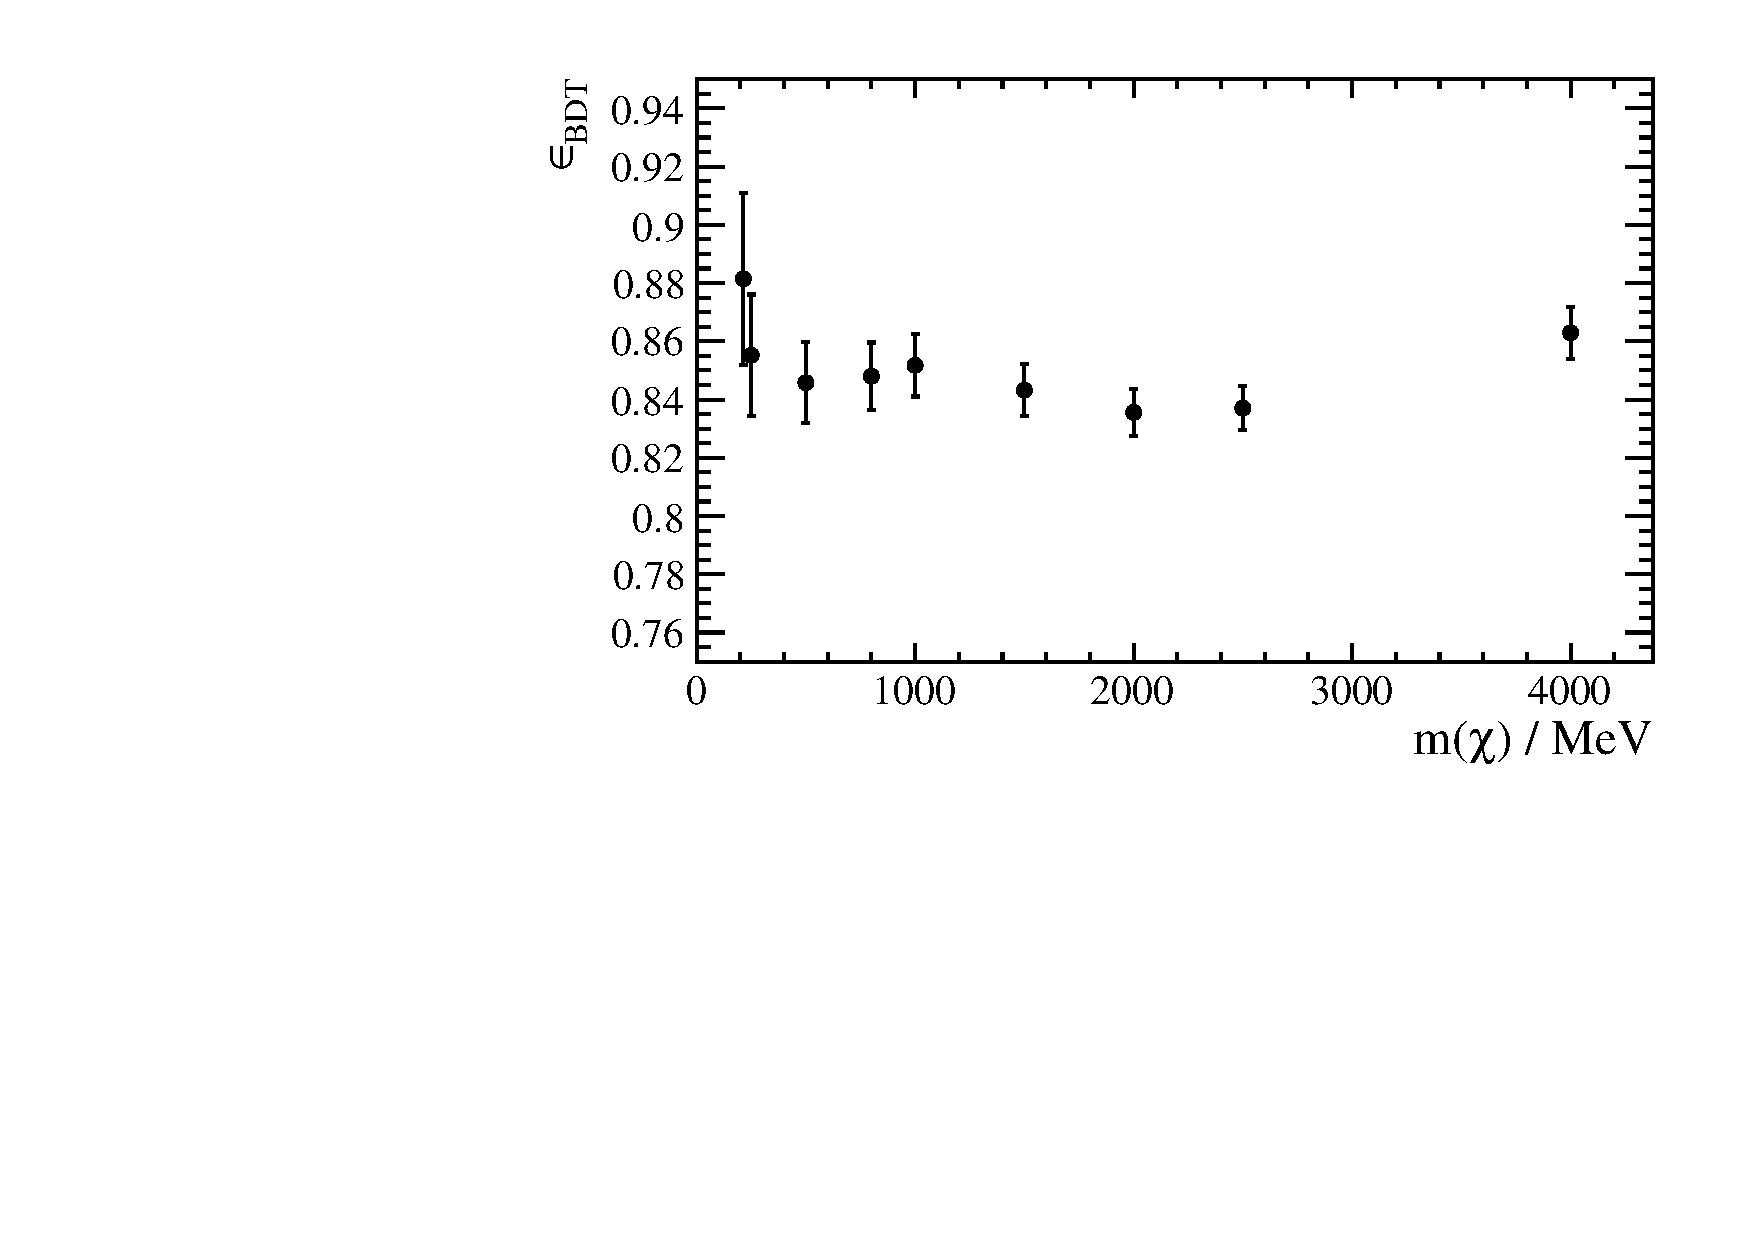
\includegraphics[width=0.48\textwidth]{mvaMassEff}
    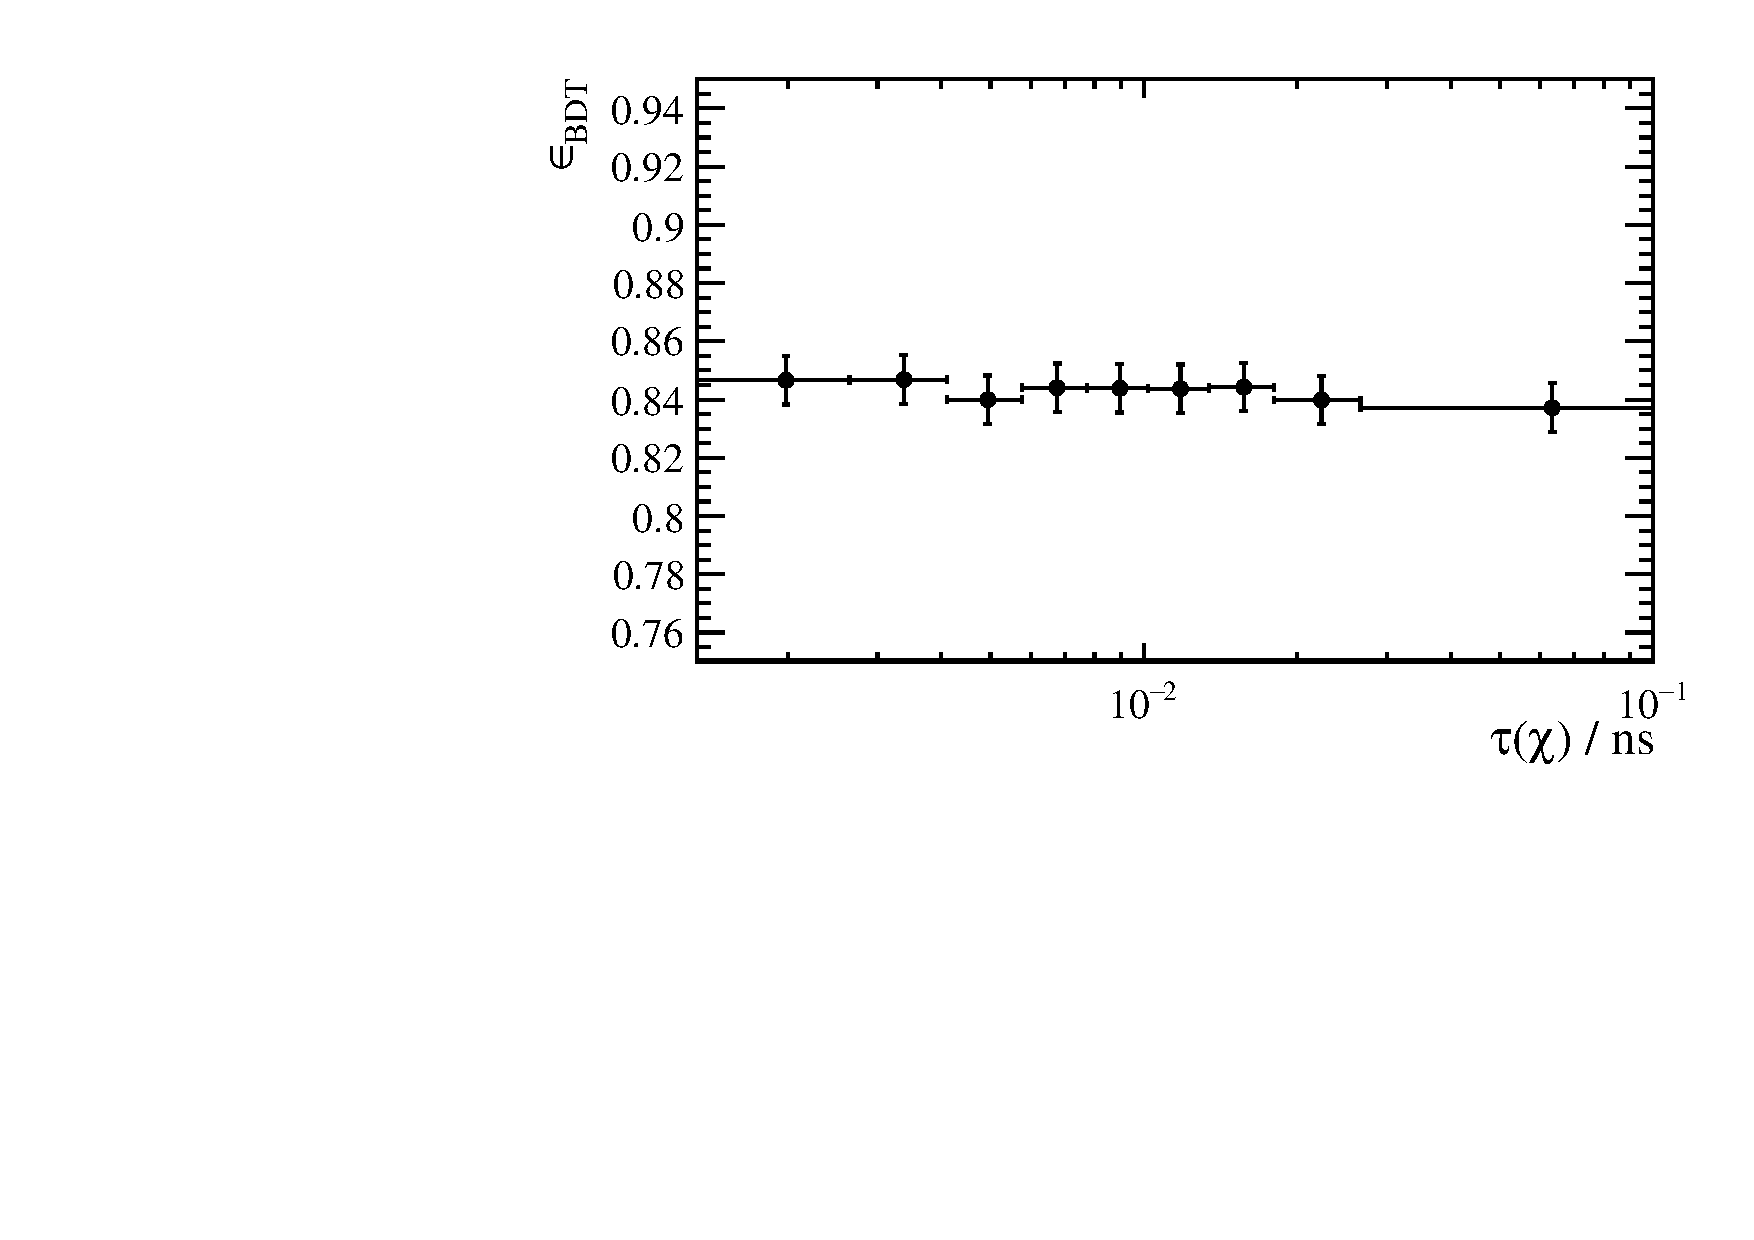
\includegraphics[width=0.48\textwidth]{anaTauEffMVA}
    \caption[Signal efficiency of the uBDT as a function of mass and lifetime]
    {
      It is observed that the efficiency of the \uBDT as a function of
      (left) \mdb and
      (right) \tdb is flat.
      Here, a cut which is \approx$85\pc$ efficient is applied.
    }
    \label{fig:db:bdtflat}
  \end{center}
\end{figure}

%\begin{equation}
  %P_\sigma = \frac{S}{\sqrt{B} + \frac\sigma2},
%\end{equation}
%where $\sigma$ is the desired level of observation, $S$ is the amount of signal, and $B$ is the
%bakground level.
%The value of $S$ is determined to be the number of signal events that pass a given cut, while $B$
%is calculated by

%to be the number of events rem
%using various simulated samples of the decay \btokstrdb, and is
%simpl
%
%a number of simulated samples of \btokstrdb, where the signal is
%simply the number of

The \uBDT cut is optimized  by maximizing
the Punzi figure-of-merit, which is defined as
\begin{equation}
  \mathrm{Punzi}_\sigma = \frac{S}{\sqrt{B} + \tfrac12\sigma},
  \label{eq:db:punzi}
\end{equation}
where $S$ and $B$ are the signal and background yields, respectively; and $\sigma$ is the desired
level of observation.
The signal and background yields are calculated as follows:
$S$ is the number of simulated signal events which survive a \uBDT cut;
$B$ is the background yield as estimated using \btokstrdb candidates
that fall outside $80\mev$ from the nominal \Bd mass~\cite{PDG2014}.
The invariant mass distributions of these candidates in data are fit to a decaying exponential,
and the background yield is taken to be the integral of this exponential within $60\mev$
(approximately $3\sigma$) of $m^\mathrm{PDG}_{\Bd}$.

The figure-of-merit is considered separately for both the prompt and displaced candidates.
The optimal working point varies from sample to sample due to the fact that the background yield
depends on $(m,\tau)$.
However, the optimal point in the prompt case is approximately $\uBDT>0.15$ for all samples, a
working point that
is approximately $85\pc$ efficient by constructing.
At this point in the displaced region, there is an estimated zero background.
This point was calculated used a value of $\sigma=5$, \Eq{eq:db:punzi}, although the result is seen
to be insensitive to its exact value.



%In \Sect{sec:strategy} it is briefly mentioned that the observed signal yields will be normalized
%with respect to the SM decay \btokstrmumu.
%Specifically the \qsq range $1.1<\qsq<6.0\gevgev$ will be used, because theoretical and
%experimental uncertainties are low in this region.
%Here, \qsq is defined to be the invariant mass of the dimuon pair, squared.







%\subsection[Mass of \Bd candidates]{Mass of $\boldsymbol{\Bd}$ candidates}
%\label{ssec:sel:massb}
%As mentioned above, all masses in this analysis are computed using {\tt DecayTreeFitter}, where the
%mass of the \Bd candidate is constrained to the world average value in the vertex fit~\cite{PDG2012}.
%The analysis is performed on all \Bd candidates that fall within $150\mev$ of the nominal \Bd
%mass~\cite{PDG2012}, where the mass is the mass from the unconstrained vertex fit (the upper sideband of
%which is used for to train the multivariate selection, which is described below).
%A tighter criteria is placed on the \Bd mass to select the final sample of candidates to use in the \db search.
